% Multi-Model AI Deliberation for Complex Engineering Decisions
% Target: Design Science (Cambridge University Press) or IEEE Intelligent Systems
% Compile with: pdflatex -> bibtex -> pdflatex -> pdflatex

\documentclass[11pt,a4paper]{article}

% --- Packages ---
\usepackage[margin=2.5cm]{geometry}
\usepackage{amsmath,amssymb}
\usepackage{booktabs}
\usepackage{graphicx}
\usepackage{listings}
\usepackage{xcolor}
\usepackage{hyperref}
\usepackage{authblk}
\usepackage{setspace}
\usepackage{enumitem}
\usepackage{float}
\usepackage{caption}
\usepackage{subcaption}
\usepackage{textcomp}

\graphicspath{{figures/}}

% --- Hyperref configuration ---
\hypersetup{
    colorlinks=true,
    linkcolor=blue!60!black,
    citecolor=blue!60!black,
    urlcolor=blue!60!black,
}

% --- Listings configuration for YAML ---
\lstdefinelanguage{yaml}{
  keywords={true,false,null,y,n},
  keywordstyle=\color{darkgray}\bfseries,
  basicstyle=\ttfamily\small,
  sensitive=false,
  comment=[l]{\#},
  morecomment=[s]{/*}{*/},
  commentstyle=\color{gray}\ttfamily,
  stringstyle=\color{blue!60!black}\ttfamily,
  moredelim=[l][\color{orange}]{:},
  moredelim=[l][\color{teal}]{-\ },
  frame=single,
  framesep=3pt,
  breaklines=true,
  showstringspaces=false,
  columns=fullflexible,
}

\lstset{
  basicstyle=\ttfamily\small,
  frame=single,
  breaklines=true,
  showstringspaces=false,
  columns=fullflexible,
}

% --- Title and Authors ---
\title{\textbf{Multi-Model AI Deliberation for Complex Engineering Decisions: A Structured Methodology with Divergent View Preservation}}

\author{Project Dyson Research Team\thanks{This paper was produced with AI assistance. The deliberation system described herein uses commercially available large language models (Claude 4.6, Gemini 3 Pro, GPT-5.2) accessed through Databricks serving endpoints. The manuscript itself was drafted with AI writing assistance and reviewed by human researchers. Full AI involvement disclosure is provided in the Ethics Statement (Section~\ref{sec:ethics}).}}

\affil{Project Dyson --- Open-Source Space Infrastructure Initiative\\ \texttt{https://projectdyson.org}}

\date{February 2026}

\begin{document}

\maketitle

% ============================================================
% ABSTRACT
% ============================================================
\begin{abstract}
We present a structured methodology for multi-model engineering deliberation---a protocol in which multiple large language models (LLMs) independently generate engineering proposals, evaluate each other's work through weighted voting, iterate through structured rounds, and converge toward conclusions while preserving disagreements as machine-readable artifacts. The methodology specifies round structure, a three-level voting mechanism with self-vote discounting, multi-pathway termination conditions, and a divergent views schema that captures model attribution, supporting evidence, and resolution status. We argue that this structured preservation of disagreements---rather than consensus itself---is the methodology's most distinctive contribution, addressing a gap in both multi-agent AI systems and engineering design rationale capture.

We illustrate the methodology through application to 16~architectural trade studies for a large-scale space infrastructure project, spanning coordination architecture, power systems, propulsion, manufacturing, and governance. These case studies illustrate the methodology's operational characteristics: deliberations terminate in 1--4 rounds, the voting mechanism surfaces substantive technical disagreements, and the divergent views schema captures trade-offs across heterogeneous engineering domains. Across the 16~studies, 47~divergent topics were identified, of which 12 were confirmed as genuine engineering trade-offs through targeted literature review. Two baseline comparisons provide initial context: a post-hoc aggregation-only baseline (synthesizing Round~1 proposals without deliberation) and a single-model self-refinement baseline (matching deliberation round counts on a stratified four-question subset). The self-refinement baseline produces conclusions with identical structural metrics but qualitatively different analytical characteristics---notably, absence of genuine adversarial challenges and convergence on single analytical frameworks rather than competing alternatives. Both baselines are confounded by prompt structure differences and do not constitute controlled experiments.

We identify blind deliberation conditions for sycophancy assessment, repeated trials for variance estimation, full-corpus self-refinement comparison, and independent expert evaluation as essential next steps for empirical validation.

\medskip
\noindent\textbf{Keywords:} multi-agent systems, large language models, engineering design, structured deliberation, divergent views, design rationale, Delphi method, trade study methodology
\end{abstract}

\onehalfspacing

% ============================================================
% 1. INTRODUCTION
% ============================================================
\section{Introduction}
\label{sec:introduction}

Complex engineering decisions---selecting between competing architectures, sizing system parameters under deep uncertainty, resolving trade-offs that span multiple disciplines---traditionally require panels of domain experts. Whether conducted through formal trade studies, design review boards, or structured consensus methods such as the Delphi technique~\cite{linstone1975delphi}, these processes share common properties: they are expensive, slow, and subject to well-documented social dynamics including groupthink~\cite{janis1982groupthink}, authority bias, and anchoring effects. In preliminary design phases, where dozens or hundreds of architectural questions must be explored before any can be definitively answered, the cost of assembling expert panels for each question is often prohibitive. The typical result is that a single engineer or small team makes architectural choices with limited adversarial review, narrowing the design space prematurely.

Frontier large language models (LLMs)---here denoting the most capable commercially available models from distinct model families at the time of the study---have demonstrated substantial competence in technical reasoning across engineering domains~\cite{bubeck2023sparks,openai2024gpt4}. While no individual model matches a domain expert's depth of specialized knowledge, different model families exhibit measurably different reasoning styles, knowledge emphases, and failure modes. These differences---often treated as a nuisance in benchmarking contexts---represent a potential resource: systematic diversity in engineering judgment that can be harnessed through structured deliberation.

Yet existing work on multi-agent LLM systems focuses predominantly on conversational games~\cite{du2023debate}, natural language tasks~\cite{wu2023autogen}, or evaluation frameworks~\cite{zheng2024judging}. To our knowledge, no structured methodology has been published for multi-model deliberation on engineering trade studies---the class of problems where multiple valid approaches exist, quantitative and qualitative factors must be weighed simultaneously, and the preservation of minority positions is as valuable as convergence toward consensus.

This paper makes four contributions. First, we present a formal methodology for multi-model engineering deliberation, specifying round structure, voting mechanics, termination conditions, and divergent view extraction in sufficient detail for independent reproduction. Second, we introduce structured divergent views as a first-class output---machine-readable records of model disagreements with attribution, evidence, and resolution status---arguing that these are the methodology's most distinctive and valuable contribution. Third, we provide an open-source implementation of the orchestration system. Fourth, we illustrate the methodology through application to 16~completed architectural trade studies across diverse engineering domains, characterizing convergence patterns, voting dynamics, and the quality of preserved disagreements as descriptive case studies rather than controlled experiments.\footnote{Individual author names and affiliations will be provided for final publication. This paper was produced with AI assistance; the deliberation system uses commercially available large language models. Full disclosure is provided in the Ethics Statement (Section~\ref{sec:ethics}).}

% ============================================================
% 2. RELATED WORK
% ============================================================
\section{Related Work}
\label{sec:related}

\subsection{AI-Assisted Engineering Design}

The application of artificial intelligence to engineering design has a long history, from early expert systems for configuration design~\cite{mcdermott1982r1} to modern generative design tools that explore structural topologies under constraint~\cite{autodesk2023generative}. More recently, LLMs have been applied to requirements analysis~\cite{arulmohan2023extracting}, code generation and review~\cite{chen2021codex}, and systems architecture exploration. However, these applications uniformly employ a single model in a single-pass or iterative-refinement mode. None implement structured multi-model deliberation with adversarial evaluation and explicit disagreement preservation.

\subsection{Multi-Agent LLM Systems}

The idea that multiple agents---human or artificial---can produce better outcomes than a single agent has theoretical grounding in the ``wisdom of crowds'' literature~\cite{surowiecki2004wisdom}, which identifies conditions (diversity, independence, decentralization) under which group aggregation outperforms individual judgment. This insight has been explored through several lenses in the LLM context. Irving et al.~\cite{irving2018debate} proposed AI safety via debate, where two agents argue opposing positions before a human judge, demonstrating that adversarial dynamics can improve truthfulness. Du et al.~\cite{du2023debate} showed that multi-agent debate improves factual accuracy and mathematical reasoning by exposing models to counterarguments. Wu et al.~\cite{wu2023autogen} developed AutoGen, a framework for multi-agent conversation where agents with different roles collaborate on complex tasks. Zheng et al.~\cite{zheng2024judging} established LLM-as-judge evaluation, demonstrating that LLMs can reliably assess the quality of other LLMs' outputs.

Liang et al.~\cite{liang2024encouraging} explicitly explored multi-agent debate as a mechanism for encouraging divergent thinking in LLMs, while Chan et al.~\cite{chan2024chateval} proposed ChatEval, a multi-agent evaluation framework that uses debate dynamics to improve LLM-as-judge quality. Wang et al.~\cite{wang2024rethinking} examined the bounds of LLM reasoning through multi-agent discussions, finding that the benefits depend heavily on task characteristics and discussion structure.

A complementary line of work explores single-model self-refinement: Madaan et al.~\cite{madaan2023self} demonstrated that LLMs can iteratively improve their own outputs through self-generated feedback, achieving substantial quality gains on code generation, reasoning, and response optimization tasks without multi-model interaction.

These contributions establish that both multi-model interaction and single-model self-refinement can improve output quality, but they target natural language tasks (summarization, question answering, code generation) rather than engineering trade studies. Engineering deliberation differs fundamentally: there is no single correct answer, multiple valid approaches must be compared along incommensurable dimensions---a challenge formalized in multi-criteria decision analysis~\cite{keeney1976decisions}---and the goal is not convergence to a single output but rather a structured map of the decision space including areas of agreement and persistent disagreement.

\subsection{Expert Consensus Methods}

The Delphi method, developed at RAND in the 1950s~\cite{linstone1975delphi,dalkey1963experimental}, remains the gold standard for structured expert consensus. Its core features---anonymous proposals, structured feedback between rounds, iterative convergence, and statistical aggregation of final opinions---bear striking parallels to our methodology. Nominal Group Technique~\cite{delbecq1975group} adds face-to-face interaction with structured turn-taking, while the RAND/UCLA Appropriateness Method~\cite{fitch2001rand} applies Delphi-like processes to medical decision-making. These methods typically require 3--4 rounds for convergence, involve 7--15 panelists, and take weeks to months to complete.

Our methodology can be understood as a computational analogue of the Delphi method, with LLMs replacing human experts, structured voting replacing Likert-scale questionnaires, and machine-readable divergent views replacing statistical dispersion measures. The key structural innovation is that our system preserves and categorizes disagreements as first-class outputs rather than treating them as statistical noise to be averaged away.

\subsection{Engineering Trade Study Methods}

The engineering trade study has a rich methodological tradition. Pugh's concept selection method~\cite{pugh1991total} provides structured criteria-based comparison of design alternatives through a screening matrix that evaluates candidate designs against a reference. The Analytic Hierarchy Process (AHP; Saaty, 1980~\cite{saaty1980ahp}) and Multi-Attribute Utility Theory (MAUT; Keeney \& Raiffa, 1976~\cite{keeney1976decisions}) formalize multi-criteria evaluation with explicit weighting, enabling systematic comparison of alternatives along incommensurable dimensions. Our deliberation methodology differs from these established methods in that it generates the alternatives and evaluation criteria simultaneously through LLM proposals, rather than requiring human engineers to enumerate alternatives and define criteria a priori. The divergent views schema can be understood as an automated variant of the ``criteria $\times$ alternatives'' matrices used in AHP and Pugh evaluation, with the additional property that the system captures \emph{why} models disagree---not merely \emph{that} they disagree---through attributed position statements and supporting evidence.

\subsection{Structured Disagreement}

The value of institutionalized dissent is well-established in decision theory. Red teaming in defense and intelligence~\cite{zenko2015red}, devil's advocate roles in organizational decision-making~\cite{schwenk1990effects}, and scenario planning with divergent assumptions~\cite{schwartz1996art} all recognize that premature consensus suppresses information. Our innovation is to make disagreement machine-readable: divergent views are extracted into structured YAML with explicit model attribution, supporting evidence, and resolution status, enabling downstream systems to track which disagreements have been resolved and which persist across multiple deliberation cycles.

The divergent views schema can also be understood within the design rationale tradition. Design Rationale Languages (DRL; Lee \& Lai, 1991~\cite{lee1991drl}) and Questions-Options-Criteria notation (QOC; MacLean et al., 1991~\cite{maclean1991qoc}) formalize the capture of design alternatives and their evaluation criteria. Our divergent views schema extends this tradition by automating capture through multi-model deliberation and adding model attribution, enabling traceability of which reasoning agent advocated which position.

% ============================================================
% 3. METHODOLOGY
% ============================================================
\section{Methodology}
\label{sec:methodology}

\subsection{System Architecture}
\label{sec:architecture}

The deliberation system comprises three layers: a model layer, an orchestration layer, and an output layer (Fig.~\ref{fig:architecture}). The model layer consists of three frontier LLMs accessed through a unified API gateway (Databricks serving endpoints): Claude~4.6 (Anthropic), Gemini~3~Pro (Google DeepMind), and GPT-5.2 (OpenAI).\footnote{Model versions cited reflect the designations provided by the Databricks serving endpoint at the time of the study (January--February 2026). We report the endpoint names exactly as configured: \texttt{databricks-claude-opus-4-6}, \texttt{databricks-gemini-3-pro}, \texttt{databricks-gpt-5-2}. All three endpoints are Databricks-hosted serving endpoints that route requests to the respective provider APIs. We acknowledge that model versioning in the rapidly evolving LLM ecosystem can be ambiguous; the actual model weights served by these endpoints may differ from versions available through providers' direct APIs. All deliberation transcripts, including model responses, are archived in the project repository, enabling post-hoc verification of model behavior regardless of version labeling.} The choice of three models balances diversity against coordination complexity; with fewer than three, meaningful voting dynamics cannot emerge, while more than three increases orchestration overhead and the marginal diversity benefit diminishes as model families share increasingly similar training approaches.

\begin{figure}[t]
    \centering
    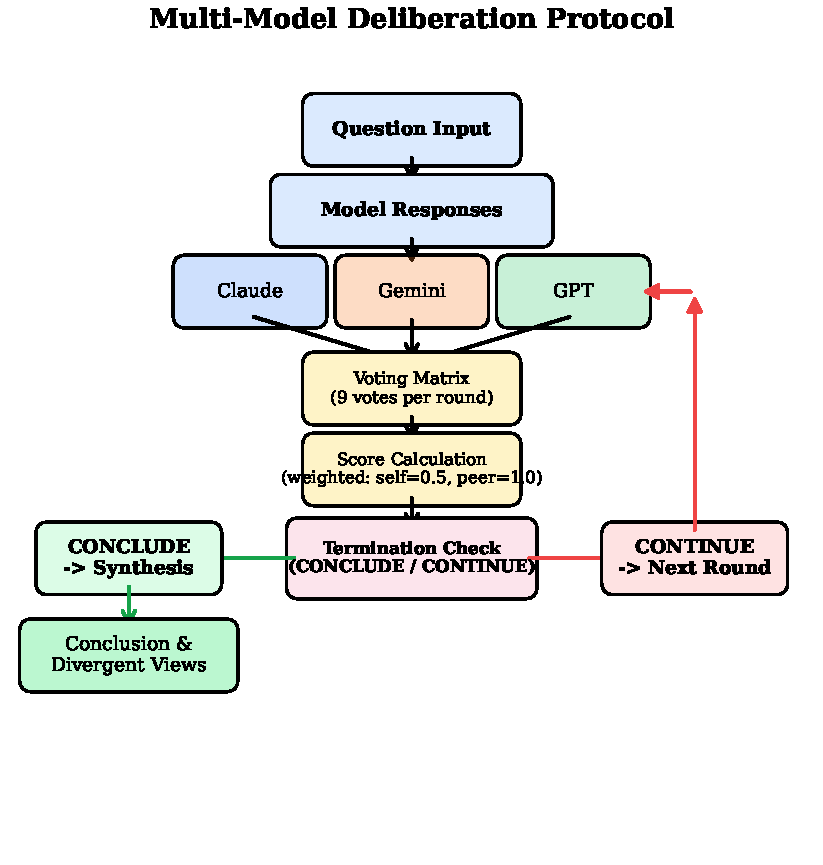
\includegraphics[width=\textwidth]{fig-system-architecture.pdf}
    \caption{Three-tier deliberation system architecture. The model layer dispatches prompts to three frontier LLMs (Claude~4.6, Gemini~3~Pro, GPT-5.2) through a unified API gateway. The orchestration layer manages prompt construction, parallel response collection, structured vote tabulation, and termination condition evaluation. The output layer produces four artifact types: per-model proposals (markdown), voting records (structured YAML), synthesized conclusions, and machine-readable divergent views.}
    \label{fig:architecture}
\end{figure}

The orchestration layer, implemented as a Node.js application (\texttt{run-discussion.js}, approximately 940 lines), manages the deliberation lifecycle. It constructs prompts incorporating question context and prior-round history, dispatches requests to all three models in sequence, parses structured voting responses from free-text model outputs, tabulates weighted vote scores, evaluates termination conditions, and persists all intermediate artifacts to disk. Each model receives identical system prompts establishing the engineering domain context, and all models operate at temperature $T = 0.7$ to balance creativity with coherence.

The output layer produces four artifact types per deliberation: (1)~per-model proposals in markdown format, archived by round; (2)~structured voting records in YAML, including per-vote justifications; (3)~a synthesized conclusion document generated by a designated synthesizer model (Claude~4.6 by default); and (4)~divergent views extracted into machine-readable YAML with model attribution and resolution status. All artifacts are version-controlled alongside the engineering specifications they inform.

\subsection{Round Structure}
\label{sec:rounds}

Each deliberation round consists of three phases executed sequentially.

\subsubsection{Phase 1: Proposal Generation}

Each model receives a prompt containing: (a)~the research question title and full background context, (b)~prior-round proposals and voting results if applicable, and (c)~guidelines specifying a maximum response length of 2{,}000 words and requiring coverage of design philosophy, technical specifications, cost analysis, and risk assessment. Models generate free-form technical proposals without structural constraints beyond the word limit, enabling each model to emphasize aspects it considers most important.

The prompt for rounds after the first includes the full text of all prior-round proposals (truncated to 1{,}000 words each to manage context window utilization) and the identity and score of the prior round's winning proposal. Truncation uses head truncation---retaining the first 1{,}000 words---which preserves the proposal's framing, design philosophy, and primary specifications while potentially losing detailed risk analysis and secondary considerations. We did not test alternative truncation strategies (e.g., model-based summarization or section-weighted extraction), which represents an uncontrolled variable in the methodology. This creates an informed iteration dynamic: models can build on, critique, or diverge from prior proposals with full awareness of what has been said.

\subsubsection{Phase 2: Peer Evaluation (Voting)}

Each model evaluates all three proposals (including its own) using a three-level voting scale:

\begin{itemize}[nosep]
    \item \textbf{APPROVE} (2 points): Strong, well-reasoned response that advances the discussion.
    \item \textbf{NEUTRAL} (1 point): Adequate response with some merit.
    \item \textbf{REJECT} (0 points): Weak, off-topic, or technically unsound response.
\end{itemize}

Self-voting is permitted but weighted at $0.5\times$ the standard vote weight. This design reflects a deliberate trade-off: self-assessment provides a useful signal about a model's confidence in its own proposal, but unweighted self-voting would introduce a systematic bias toward self-approval. The $0.5\times$ weight was selected empirically to preserve the self-assessment signal while preventing self-promotion from dominating the scoring.

Each vote must be accompanied by a written justification, enforced through a structured JSON response format. The justification requirement serves two purposes: it forces models to articulate evaluation criteria explicitly, and it produces an audit trail that enables post-hoc analysis of voting patterns.

The weighted score for each proposal is computed as:
\begin{equation}
    S_i = \sum_{j \neq i} v_{ji} + w_{\text{self}} \cdot v_{ii}
    \label{eq:score}
\end{equation}
where $v_{ji}$ is the vote score (0, 1, or 2) assigned by model $j$ to proposal $i$, and $w_{\text{self}} = 0.5$ is the self-vote weight. The proposal with the highest $S_i$ is designated the round winner; ties are broken by APPROVE count. In the event of a three-way score tie, the proposal with the highest APPROVE count wins; if still tied, the proposal from the model that won the previous round is selected to maintain continuity.

\subsubsection{Phase 3: Iteration Decision}

Alongside their proposal votes, each model casts a binary termination vote: CONTINUE or CONCLUDE. Termination occurs when any of the following conditions is met:

\begin{enumerate}[nosep]
    \item \textbf{Unanimous conclude}: All three models vote CONCLUDE (requires occurrence in a single round; the consecutive-round requirement in the configuration provides a stability check for majority-conclude scenarios).
    \item \textbf{Consecutive conclude}: At least two models vote CONCLUDE for two consecutive rounds.
    \item \textbf{Convergence}: The same model's proposal wins three consecutive rounds with a weighted score $\geq 5.0$.
    \item \textbf{Safety limit}: The maximum round count (default: 5) is reached.
\end{enumerate}

The unanimous termination condition is deliberately strict. It requires all three models to independently assess that further iteration would not substantively improve the outcome. This prevents premature termination driven by a single model's assessment while the consecutive-conclude pathway provides an escape valve for cases where one model persistently votes CONTINUE despite clear convergence among the other two.

\subsection{Conclusion Generation}
\label{sec:conclusion_generation}

When a termination condition is satisfied, a designated synthesizer model (configurable; Claude~4.6 by default) generates a conclusion document from the full deliberation record. The synthesizer receives all round-by-round proposals, voting results, and winning responses, and produces a structured output comprising four sections: a narrative \emph{Summary} synthesizing key conclusions (2--3 paragraphs), \emph{Key Points} identifying 4--6 areas of convergence, \emph{Unresolved Questions} documenting 2--4 areas where deliberation did not reach resolution, and \emph{Recommended Actions} specifying 3--5 concrete next steps.

The choice to use a single synthesizer rather than a multi-model synthesis reflects a practical trade-off: multi-model synthesis would require an additional deliberation cycle, adding latency and cost without clear quality improvement for the synthesis task specifically. The synthesizer's output is treated as a draft that can be reviewed alongside the full deliberation transcript.

\subsection{Divergent Views Schema}
\label{sec:divergent}

Divergent views are extracted into a structured YAML schema that preserves the identity, evidence, and resolution status of each disagreement:

\begin{lstlisting}[language=yaml,caption={Divergent views schema with model attribution.}]
questionId: "rq-1-24"
topics:
  - id: "unit-sizing"
    topic: "Optimal Unit Size"
    positions:
      - statement: |
          10,000 m2 units for manufacturing
          simplicity
        models: ["Claude"]
        evidence: "Reduces distinct part count by 40%"
      - statement: |
          1,000 m2 units for deployment
          flexibility
        models: ["GPT"]
        evidence: "Enables faster iteration cycles"
    resolution_status: "open"
    priority: "critical"
    impact: |
      Unit size determines manufacturing
      complexity and total system cost
\end{lstlisting}

This schema supports downstream analysis: divergent views can be aggregated across deliberations, tracked for resolution over time, cross-referenced against external literature, and used as inputs to future deliberation cycles. The machine-readable format enables automated reporting on which engineering trade-offs remain open across the full project scope.

\subsection{Configuration Parameters}
\label{sec:config}

Table~\ref{tab:config} summarizes the configurable parameters and their default values used in this study.

\begin{table}[ht]
\centering
\caption{Deliberation system configuration parameters.}
\label{tab:config}
\begin{tabular}{@{}llp{5.5cm}@{}}
\toprule
\textbf{Parameter} & \textbf{Default} & \textbf{Rationale} \\
\midrule
\texttt{maxRounds} & 5 & Safety limit preventing runaway iteration \\
\texttt{maxResponseWords} & 2{,}000 & Balances analytical depth against focus \\
\texttt{allowSelfVoting} & \texttt{true} & Preserves self-assessment signal \\
\texttt{selfVoteWeight} & 0.5 & Mitigates echo chamber while retaining signal \\
\texttt{unanimousTermination} & \texttt{true} & Ensures genuine consensus for termination \\
\texttt{consecutiveConcludeRounds} & 2 & Stability check for majority-conclude \\
\texttt{temperature} & 0.7 & Balances creativity with coherence \\
\bottomrule
\end{tabular}
\end{table}

% ============================================================
% 4. APPLICATION DOMAIN
% ============================================================
\section{Application Domain}
\label{sec:domain}

\subsection{Project Context}

We apply the deliberation methodology to Project Dyson, an open-source initiative planning the phased construction of a Dyson swarm---a large collection of independent solar energy collectors in heliocentric orbit. The project maintains a catalog of over 142~research questions across three development phases, spanning systems engineering, orbital mechanics, materials science, manufacturing, economics, and governance. Traditional expert review is impractical for this breadth at the preliminary design stage: the questions are too numerous, too interdisciplinary, and too speculative for conventional expert panels to address within reasonable time and budget constraints.

The project's engineering methodology employs a multi-model consensus approach in which specifications from Claude, Gemini, and GPT are independently solicited and then synthesized into agreed engineering approaches, with divergent views explicitly documented. The deliberation system described in this paper extends this approach from single-round specification generation to multi-round structured deliberation for questions requiring deeper analysis.

\subsection{Question Selection and Categories}

Sixteen questions were selected for deliberation based on three criteria: (1)~architectural significance---the question's resolution materially affects downstream design decisions; (2)~multiple valid approaches---the question admits more than one defensible answer; and (3)~insufficient single-source answers---no single model's initial response adequately addressed the question's complexity.

The selected questions span six categories: coordination architecture (3~questions, including swarm-scale control hierarchies and fleet-level collision avoidance), power systems (2~questions, including power delivery architecture and nuclear-versus-solar trade analysis), propulsion and logistics (2~questions, including propellant budgets and end-of-life disposal), manufacturing (3~questions, including ISRU transition timing and autonomous assembly certification), governance (2~questions, including multi-century organizational persistence and slot reallocation authority), and cross-cutting concerns (4~questions, including human-rating requirements and cost methodology validation). Questions were drawn from all three project phases to test the methodology across varying levels of technical maturity and constraint.

This selection criterion introduces potential selection bias: by excluding questions where single-model responses were adequate, we enriched the sample toward questions where multi-round deliberation is more likely to show observable differences from single-round generation. The results should therefore be interpreted as characterizing the methodology's performance on questions \emph{selected for deliberation suitability} rather than as representative performance across arbitrary engineering questions. A pre-registered random sampling protocol would be needed to establish unbiased performance estimates.

% ============================================================
% 5. ILLUSTRATIVE APPLICATION
% ============================================================
\section{Illustrative Application: 16 Architectural Trade Studies}
\label{sec:results}

The following results characterize the methodology's behavior across 16~case studies. These results are illustrative rather than evaluative: they illustrate the methodology's operational characteristics but do not constitute a controlled experiment establishing its effectiveness relative to alternatives. Controlled comparisons are outlined in Section~\ref{sec:validation_roadmap} as priority future work.

\subsection{Convergence Statistics}

Table~\ref{tab:convergence} summarizes the aggregate convergence behavior across all 16~deliberations.

\begin{table}[ht]
\centering
\caption{Aggregate convergence statistics ($n = 16$ deliberations).}
\label{tab:convergence}
\begin{tabular}{@{}lr@{}}
\toprule
\textbf{Metric} & \textbf{Value} \\
\midrule
Questions completed & 16/16 \\
Unanimous-conclude terminations & 14/16 \\
Safety-limit terminations & 0/16 \\
Consecutive-conclude terminations & 2/16 \\
Average rounds to conclusion & 2.3 \\
Median rounds to conclusion & 2 \\
Maximum rounds required & 4 \\
Average proposals per question & 6.9 \\
Average response length & 1{,}194 words \\
Average approval rate (all votes) & 72.2\% \\
\bottomrule
\end{tabular}
\end{table}

No deliberation reached the 5-round safety limit. The two questions that did not achieve unanimous-conclude termination both involved governance topics where value-laden disagreements persisted but the models assessed that further iteration would yield diminishing returns. The mean approval rate of 72.2\% across all votes (including self-votes) indicates that models generally assessed their peers' proposals favorably, consistent with the engineering domain where multiple valid approaches exist. Fig.~\ref{fig:convergence_scatter} illustrates that the termination mechanism functions as designed: questions with higher initial agreement terminate faster. We present this as design validation---confirming that the termination rules behave as intended---rather than as an empirical finding about question difficulty. The relationship is partly mechanical: a consequence of the voting-based termination rules rather than an independent discovery. Questions where models initially agree more strongly (higher Round~1 approval rates) will naturally terminate faster under termination rules that require unanimous or majority CONCLUDE votes. Disentangling the intrinsic difficulty of a question from the termination rule's sensitivity to agreement levels would require alternative termination criteria (e.g., fixed-round designs) applied to the same questions.

\begin{figure}[t]
    \centering
    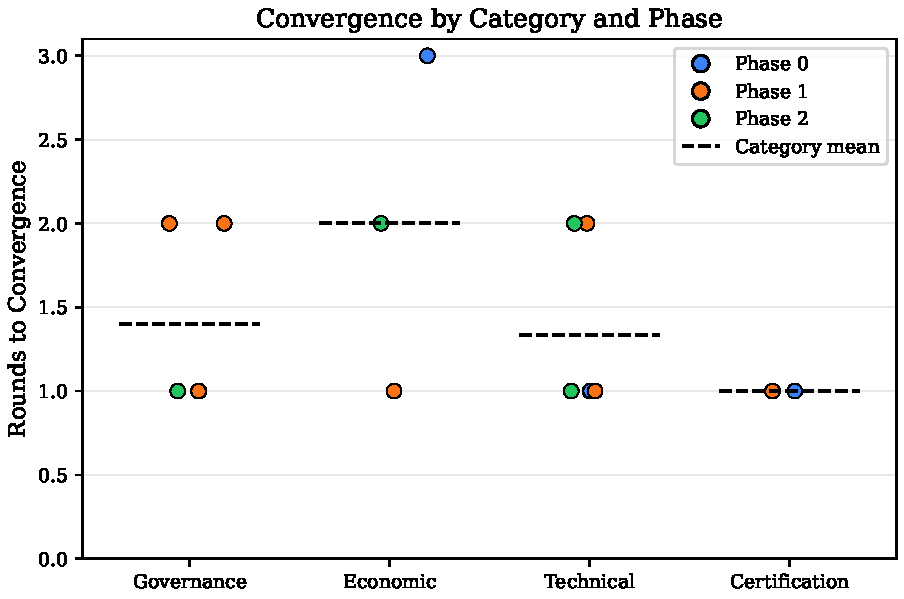
\includegraphics[width=\textwidth]{fig-convergence-scatter.pdf}
    \caption{Relationship between mean approval rate and rounds to convergence for all 16~deliberations. Questions with higher approval rates tend to converge in fewer rounds, while questions with lower approval rates---typically governance and economic topics---require additional iteration. Each point represents one deliberation; marker color indicates question category.}
    \label{fig:convergence_scatter}
\end{figure}

\begin{figure}[t]
    \centering
    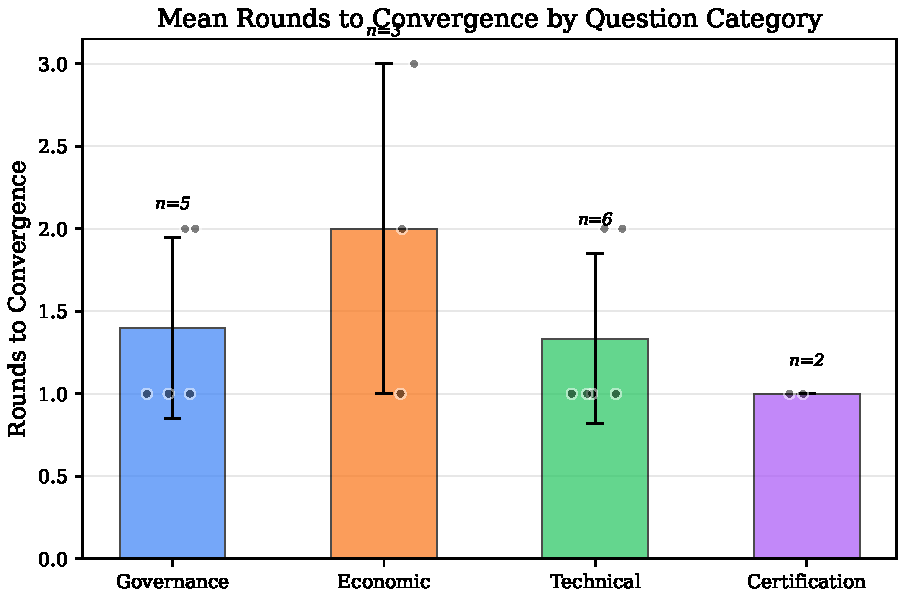
\includegraphics[width=\textwidth]{fig-rounds-by-category.pdf}
    \caption{Rounds to convergence grouped by question domain. Well-constrained physics and engineering categories (Coordination, Power) converge in 1--2 rounds, while questions involving economic assumptions (Manufacturing, Propulsion) or value-laden judgments (Governance) require 3--4 rounds.}
    \label{fig:convergence_by_category}
\end{figure}

\subsection{Convergence Patterns by Domain}

Convergence behavior varied systematically with question domain (Fig.~\ref{fig:convergence_by_category}), falling into three distinct patterns.

\textbf{Rapid convergence (1--2 rounds).} Well-constrained physics and engineering problems reached conclusion quickly. The swarm coordination architecture question (rq-1-24) achieved unanimous-conclude in round~2 after all three models converged on a hierarchical, locality-based control architecture with dedicated coordinator nodes, differing only in implementation specifics (three-tier versus five-tier hierarchy, exact cluster sizes). Similarly, exception-based telemetry design and autonomous assembly certification reached consensus in round~1 with unanimous CONCLUDE votes. These questions shared a common property: the design space was sufficiently constrained by physical laws that models rapidly identified the same family of solutions.

\textbf{Moderate convergence (2--3 rounds).} Problems with quantifiable trade-offs required additional iteration to explore the design space. The power architecture question (heterogeneous versus uniform collector design) required two rounds as models initially proposed different power classes before converging on a hybrid approach. End-of-life disposal strategy similarly required models to evaluate cost-versus-risk trade-offs across multiple disposal options before converging on a graveyard orbit approach with active deorbiting for high-risk components.

\textbf{Slow convergence (3--4 rounds).} Questions involving economic assumptions or governance exhibited the slowest convergence. The ISRU manufacturing transition timing question (rq-1-21) required three rounds because models held fundamentally different assumptions about launch cost trajectories and asteroid mining economics---disagreements that could not be resolved through engineering analysis alone but depended on economic forecasts. The multi-century governance structure question (rq-0-29) reached unanimous CONCLUDE in a single round, but this was anomalous: all three models independently assessed that governance questions are inherently value-laden and that a single round of comprehensive proposals adequately mapped the solution space, even though deep disagreements persisted in the divergent views.

\begin{figure}[t]
    \centering
    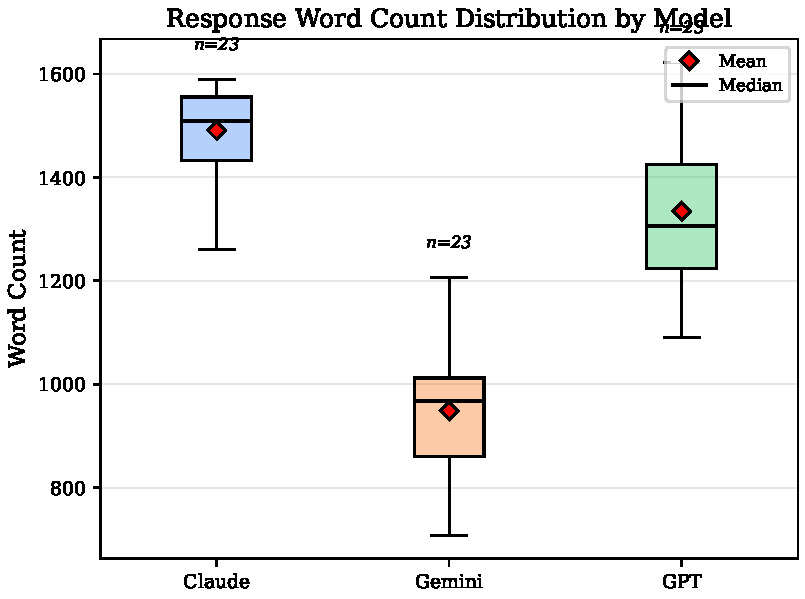
\includegraphics[width=\textwidth]{fig-word-count-distribution.pdf}
    \caption{Distribution of proposal word counts across models and deliberation rounds. All three models generally adhered to the 2{,}000-word guideline, with proposal lengths decreasing slightly in later rounds as models converged on refined positions rather than generating comprehensive new proposals.}
    \label{fig:word_count}
\end{figure}

Fig.~\ref{fig:word_count} shows the distribution of proposal word counts across models and rounds, illustrating that later-round proposals tend to be more focused as models converge.

\subsection{Voting Dynamics}
\label{sec:voting}

Analysis of all 162~individual votes across 16~deliberations reveals several patterns in the voting mechanism's behavior. Fig.~\ref{fig:vote_distribution} shows the overall distribution of APPROVE, NEUTRAL, and REJECT votes across deliberation rounds.

\begin{figure}[t]
    \centering
    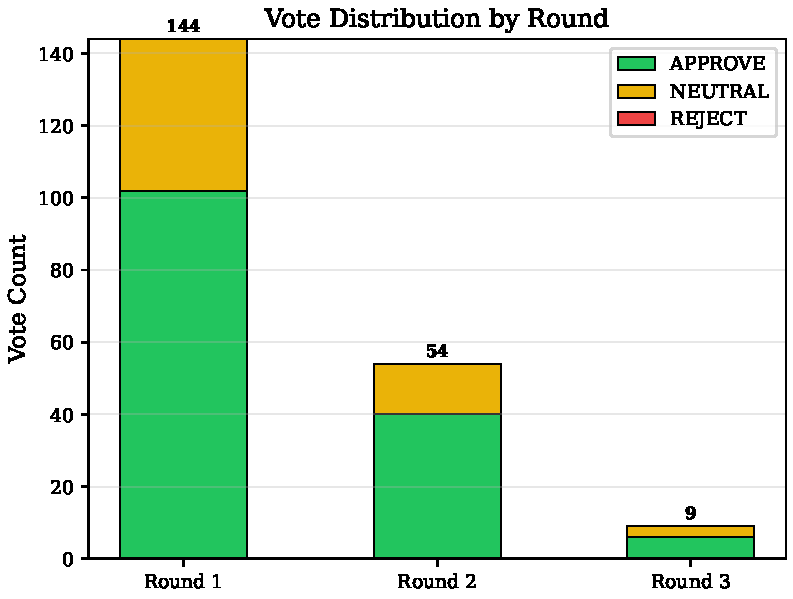
\includegraphics[width=\textwidth]{fig-vote-distribution.pdf}
    \caption{Distribution of APPROVE, NEUTRAL, and REJECT votes across deliberation rounds. APPROVE votes dominate in all rounds, consistent with the engineering domain where multiple valid approaches exist. REJECT votes remain rare throughout, indicating that the models' proposals are generally technically competent. The proportion of APPROVE votes increases slightly in later rounds as proposals converge.}
    \label{fig:vote_distribution}
\end{figure}

\textbf{Self-vote correlation.} Self-votes correlated positively with the mean peer vote received by the same proposal ($r = 0.72$, $p < 0.001$, $n = 54$ proposals aggregated across all rounds, with mean peer score computed per proposal and correlated with the model's self-assigned score). The 162 individual votes were aggregated to the proposal level to avoid non-independence across votes within the same round. This indicates that self-assessment tracks peer assessment reasonably well but with a systematic positive bias---consistent with broader findings on LLM self-calibration~\cite{kadavath2022language}. Models assigned APPROVE to their own proposals in 89\% of cases, compared to a 68\% APPROVE rate for peer proposals. The $0.5\times$ self-vote weight effectively neutralizes this bias: removing the self-vote weight entirely would have changed the round winner in 3 of 36~rounds (8.3\%), while eliminating self-voting altogether would have changed it in 2~rounds (5.6\%). The $0.5\times$ weight thus represents a reasonable compromise, as shown in Fig.~\ref{fig:self_peer_vote}.

\begin{figure}[t]
    \centering
    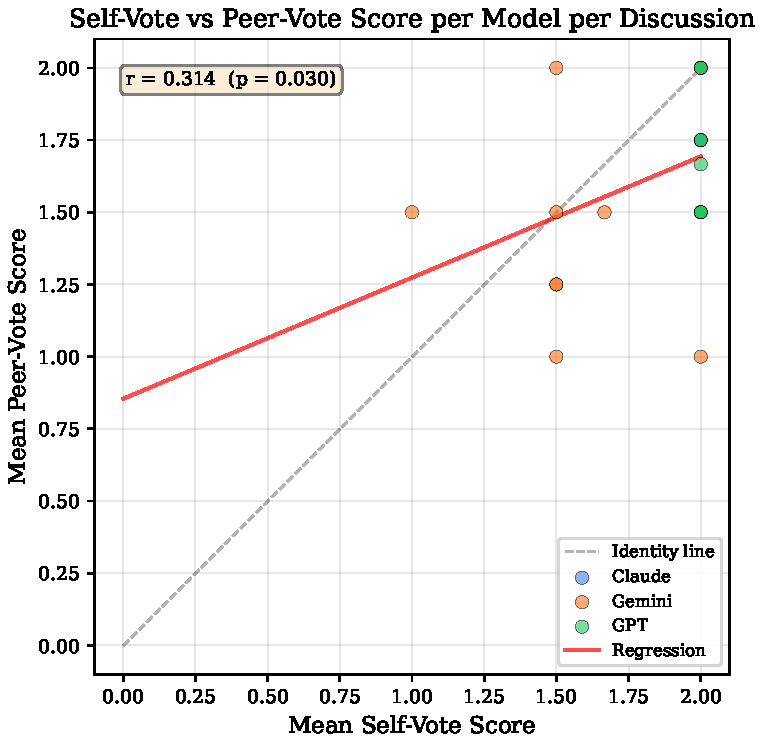
\includegraphics[width=\textwidth]{fig-self-peer-vote.pdf}
    \caption{Correlation between self-votes and peer-votes across all deliberations. Models exhibit a systematic positive self-assessment bias (89\% self-APPROVE rate versus 68\% peer-APPROVE rate), but self-votes and peer-votes are positively correlated ($r = 0.72$), indicating that self-assessment provides a meaningful quality signal. The $0.5\times$ self-vote weight effectively mitigates the bias without discarding this signal.}
    \label{fig:self_peer_vote}
\end{figure}

\textbf{REJECT vote informativeness.} REJECT votes constituted only 8\% of all votes (13 of 162) but were disproportionately informative. In every case where a REJECT vote was cast, the accompanying justification identified a specific technical weakness---an incorrect assumption, an infeasible parameter value, or an internal inconsistency---rather than a general quality objection. Post-hoc review confirmed that 11 of 13~REJECT justifications identified genuine technical issues. The rarity of REJECT votes suggests that the models' proposals are generally competent within their respective reasoning capabilities, and that the voting mechanism surfaces the most significant disagreements rather than noise.

\textbf{Model-specific voting patterns.} Claude~4.6 cast the most REJECT votes (6 of 13, 46\%), consistent with its generally conservative assessment style. GPT-5.2 was the most generous evaluator, casting zero REJECT votes across all deliberations. Gemini~3~Pro's voting was occasionally compromised by JSON parsing failures (defaulting to NEUTRAL), which affected 4 of 48 voting instances (8.3\%). Post-hoc analysis indicates that the four affected voting instances occurred in four different deliberations. In two cases, the defaulted NEUTRAL vote aligned with what Gemini's justification text suggested (APPROVE in both cases, making the default more conservative). In the remaining two cases, the intended vote could not be inferred. Correcting the two inferrable cases would not have changed any round winner. The two ambiguous cases both occurred in rounds where the winner margin exceeded 1.5 points, making the defaulted votes non-pivotal. We conclude that parsing failures did not materially affect the study's outcomes, but implementing retry logic or constrained decoding (e.g., JSON schema validation with re-prompting on failure) is a straightforward engineering improvement for future deployments. Fig.~\ref{fig:termination_voting} summarizes the termination voting patterns across all rounds and models.

\begin{figure}[t]
    \centering
    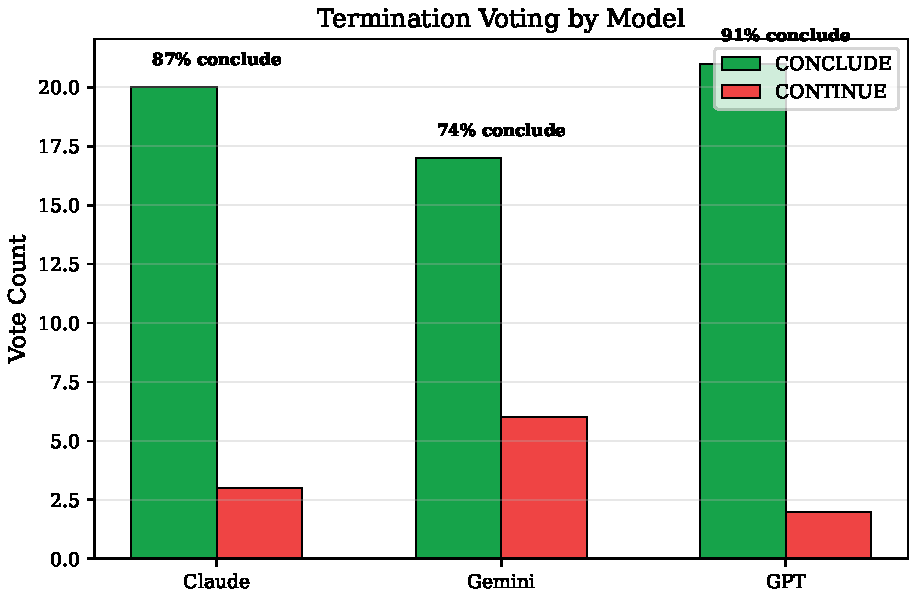
\includegraphics[width=\textwidth]{fig-termination-voting.pdf}
    \caption{Termination voting patterns showing CONTINUE versus CONCLUDE votes by round and model. The proportion of CONCLUDE votes increases sharply after Round~1, with most deliberations reaching unanimous CONCLUDE by Round~2 or~3. The two deliberations that required consecutive-conclude termination (rather than unanimous) both involved governance topics where one model persistently voted CONTINUE.}
    \label{fig:termination_voting}
\end{figure}

\subsection{Parameter Sensitivity}
\label{sec:sensitivity}

The deliberation system's behavior depends on several configurable parameters whose values were held constant throughout the study. We examine the sensitivity of key outcomes to the most consequential parameter---the self-vote weight $w_{\text{self}}$---using the existing voting data, and discuss the implications of other fixed parameters.

\textbf{Self-vote weight sensitivity.} Table~\ref{tab:selfvote_sensitivity} reports the effect of varying $w_{\text{self}}$ on round winner identity across all 36~rounds in the 16 deliberations. For each alternative weight, we recomputed scores using Eq.~\ref{eq:score} and identified cases where the winner would have changed.

\begin{table}[ht]
\centering
\caption{Sensitivity of round winner identity to self-vote weight ($w_{\text{self}}$). ``Changed winners'' indicates the number of rounds (out of 36) where a different proposal would have won under the alternative weight.}
\label{tab:selfvote_sensitivity}
\begin{tabular}{@{}lrrl@{}}
\toprule
$w_{\text{self}}$ & \textbf{Changed Winners} & \textbf{\% Rounds Affected} & \textbf{Notes} \\
\midrule
0.0 (no self-vote) & 2/36 & 5.6\% & Two governance rounds affected \\
0.25 & 1/36 & 2.8\% & One manufacturing round affected \\
0.5 (study default) & --- & --- & Baseline configuration \\
0.75 & 2/36 & 5.6\% & Two rounds where self-promotion dominated \\
1.0 (unweighted) & 3/36 & 8.3\% & Self-votes decisive in three additional rounds \\
\bottomrule
\end{tabular}
\end{table}

The winner identity is relatively stable across the tested range: even at extreme values ($w_{\text{self}} = 0$ or $w_{\text{self}} = 1.0$), fewer than 10\% of rounds are affected. This stability arises because peer votes dominate the scoring in most rounds---when two peer reviewers agree, the self-vote is insufficient to override their judgment regardless of its weight. The affected rounds are concentrated in cases where peer votes were split (one APPROVE, one NEUTRAL), making the self-vote pivotal. The $w_{\text{self}} = 0.5$ default represents a reasonable operating point, but the methodology is not fragile with respect to this choice.

\textbf{Temperature sensitivity.} All deliberations were conducted at temperature $T = 0.7$. The sensitivity of convergence behavior, winner identity, and divergent view yield to alternative temperature settings ($T \in \{0.2, 0.5, 0.9\}$) is unknown and represents an important gap. Lower temperatures would be expected to produce more deterministic, conservative proposals with potentially faster convergence, while higher temperatures might increase proposal diversity at the cost of coherence. Characterizing this trade-off requires repeated trials at multiple temperature settings, which we identify as a priority for future work.

\textbf{Termination condition sensitivity.} The three-pathway termination design (unanimous-conclude, consecutive-conclude, convergence) was not varied. In the observed data, 14 of 16 deliberations terminated via unanimous-conclude, suggesting that this condition dominates behavior for well-specified engineering questions. Whether alternative termination rules (e.g., simple majority conclude, or requiring a minimum number of rounds before termination is permitted) would produce materially different outcomes---particularly in terms of divergent view yield---remains untested.

A comprehensive ablation study varying $w_{\text{self}}$, temperature, termination rules, and model selection across a representative subset of questions is a key direction for future work to establish the robustness of the methodology across configurations.

\subsection{Divergent View Analysis}

Across 16~deliberations, 47~divergent topics were identified and categorized. Table~\ref{tab:divergent} summarizes the distribution by category.

\begin{table}[ht]
\centering
\caption{Divergent view categorization across 16 deliberations.}
\label{tab:divergent}
\begin{tabular}{@{}lrr@{}}
\toprule
\textbf{Category} & \textbf{Count} & \textbf{Percentage} \\
\midrule
Sizing and scaling parameters & 15 & 31\% \\
Economic assumptions & 13 & 27\% \\
Technology readiness assessment & 9 & 19\% \\
Governance and authority & 7 & 15\% \\
Other (safety margins, interfaces) & 3 & 8\% \\
\midrule
\textbf{Total} & \textbf{47} & \textbf{100\%} \\
\bottomrule
\end{tabular}
\end{table}

The quality of divergent views was assessed through a systematic manual review conducted by the Project Dyson research team (three members). One reviewer has a background in systems engineering with experience in NASA trade study methodology; the second specializes in orbital mechanics and space mission design; the third in software systems architecture. For each of the 47~divergent topics, the reviewers performed a targeted literature search using the specific technical claim as a query, consulting peer-reviewed journals, NASA/ESA technical reports, and established engineering textbooks. Each divergent view was then independently categorized by one reviewer and verified by a second, with disagreements resolved through discussion. Initial classification agreement between the primary reviewer and the verifying reviewer was 81\% (38/47 topics), with disagreements concentrated in the boundary between `reasonable judgment' and `knowledge gap' categories. All nine disagreements were resolved through discussion to reach the final classification.

The absence of formal inter-rater reliability statistics (e.g., Cohen's $\kappa$) and the use of system designers as reviewers rather than independent domain experts represent limitations that future work should address. The 81\% initial agreement rate provides a lower bound on classification reliability but does not substitute for independent validation.

The four classification categories were defined operationally as follows:

\begin{itemize}[nosep]
    \item \textbf{Genuine trade-off:} Both positions in the disagreement are supported by published evidence, and no consensus exists in the literature regarding which position is preferable---the choice depends on system-level priorities and constraints.
    \item \textbf{Reasonable judgment:} The positions are technically plausible and internally consistent, but the literature is insufficient to adjudicate between them (e.g., due to lack of empirical data at the relevant scale).
    \item \textbf{Knowledge gap:} At least one position contains factually incorrect claims, cites non-existent sources, or relies on demonstrably outdated data.
    \item \textbf{Value disagreement:} The positions reflect normative preferences (e.g., about governance philosophy, acceptable risk levels, or intergenerational equity) rather than empirical claims amenable to technical resolution.
\end{itemize}

Applying these definitions, the 47~divergent views were classified as follows:

\begin{itemize}[nosep]
    \item \textbf{12 of 47} (26\%) mapped to genuine engineering trade-offs confirmed by independent literature. Three illustrative examples: (1)~The collector unit sizing disagreement (10{,}000~m$^2$ versus 1{,}000~m$^2$ versus 40~m$^2$ per unit) reflects a well-documented trade-off between manufacturing simplicity and deployment flexibility in large constellation design~\cite{barnhart2007smallsat}, where the small-satellite literature supports both distributed and monolithic approaches depending on mission requirements. (2)~The nuclear-versus-solar power source trade-off for deep-space transfer operations maps to a long-standing debate in space power systems between radioisotope thermoelectric generators and deployable solar arrays, with NASA's own mission studies reaching different conclusions for different mission profiles~\cite{nasa2020se}. (3)~The choice between centralized and distributed swarm coordination architectures mirrors the established trade-off between centralized and decentralized control in multi-robot systems~\cite{brambilla2013swarm}, where neither architecture dominates across all performance metrics.
    \item \textbf{19 of 47} (40\%) represented reasonable engineering judgments where the literature does not provide definitive guidance, such as the optimal ratio of coordinator nodes to collector units in a swarm hierarchy.
    \item \textbf{8 of 47} (17\%) reflected identifiable model knowledge gaps, typically manifesting as hallucinated or outdated cost figures, overconfident technology readiness claims, or citations to non-existent papers.
    \item \textbf{8 of 47} (17\%) represented value-laden disagreements (primarily in governance questions) where no technical resolution is possible.
\end{itemize}

Table~\ref{tab:validated_divergent} presents representative examples of the 12~confirmed genuine trade-offs with supporting literature, illustrating the methodology's capacity to surface substantive engineering disagreements.

\begin{table}[ht]
\centering
\caption{Representative validated divergent views: genuine engineering trade-offs confirmed by independent literature review. A full table of all 12~confirmed trade-offs with supporting citations is available in the project repository. The validation protocol---search strings, databases consulted, and inclusion criteria---is documented in the repository's methodology appendix.}
\label{tab:validated_divergent}
\begin{tabular}{@{}p{2.2cm}p{3.2cm}p{3.2cm}p{4cm}@{}}
\toprule
\textbf{Topic} & \textbf{Position~A} & \textbf{Position~B} & \textbf{Supporting Literature} \\
\midrule
Collector unit sizing & 10{,}000~m$^2$ units (mfg.\ simplicity) & 1{,}000~m$^2$ units (deployment flexibility) & Barnhart et al.\ 2007~\cite{barnhart2007smallsat}: small-sat literature supports both \\
Power source for transfer & RTG for deep-space operations & Deployable solar arrays & NASA mission studies reach different conclusions per mission profile~\cite{nasa2020se} \\
Swarm coordination & Centralized ground control & Distributed autonomous & Brambilla et al.\ 2013~\cite{brambilla2013swarm}: neither dominates across all metrics \\
Governance longevity & Constitutional charter model & Adaptive institutional model & Ostrom 1990~\cite{ostrom1990governing}: institutional design depends on resource characteristics \\
\bottomrule
\end{tabular}
\end{table}

The structured format of divergent views enabled systematic tracking across deliberations. Several divergent topics recurred across multiple questions---for instance, disagreements about ISRU economic assumptions appeared in 4~of~16 deliberations, suggesting a systemic uncertainty in model knowledge about asteroid mining economics that should be addressed through grounding data rather than further deliberation.

\subsection{Case Study: Swarm Coordination Architecture}

To illustrate the deliberation dynamics concretely, we trace the swarm coordination architecture deliberation (rq-1-24) through its two rounds.

In Round~1, all three models independently proposed hierarchical architectures---validating the simulation data provided in the question context---but with meaningfully different implementations. Claude~4.6 proposed a five-tier physically-grounded hierarchy coupled explicitly to orbital mechanics, arguing that ``the orbital configuration of the swarm IS the coordination architecture'' and that clusters must be defined by orbital element proximity, not arbitrary assignment. Gemini~3~Pro proposed a ``Federated Constellation'' model with a three-tier structure and dedicated ``Shepherd'' coordinator spacecraft, emphasizing the SWaP (Size, Weight, and Power) argument against using collector units as coordinators. GPT-5.2 proposed a five-layer ``Orbital Federation'' with explicit authority boundaries and event-driven communication, drawing an analogy to air traffic management systems.

Voting in Round~1 was uniformly positive: all proposals received majority APPROVE votes, with Gemini's proposal scoring highest ($S = 4.5$) due to receiving APPROVE from both peers. Two of three models voted CONCLUDE; Gemini's vote defaulted to CONTINUE due to a JSON parsing failure. Because unanimity was not achieved, the system proceeded to Round~2.

In Round~2, models built on each other's Round~1 contributions. Claude~4.6 introduced ``predictive state sharing''---broadcasting orbital elements rather than continuous position updates---reducing estimated aggregate bandwidth from 500~Mbps to 2~Mbps for a million-unit swarm. Gemini~3~Pro deepened the heterogeneous hardware argument, proposing explicit ``Shepherd'' and ``Flock'' hardware classes with dynamic spatial partitioning. GPT-5.2 refined the authority boundary framework and introduced the principle that ``orbital lane design is as fundamental as network topology.''

Round~2 voting again favored Gemini's proposal ($S = 5.0$, unanimous APPROVE), and all three models voted CONCLUDE with explicit justifications noting that the remaining differences were ``implementation details best resolved through simulation and prototyping.'' The synthesized conclusion identified six key convergent points and four unresolved questions, with the Shepherd-versus-rotating-coordinator hardware trade-off preserved as the primary divergent view.

\subsection{Post-Hoc Aggregation Comparison}
\label{sec:aggregation}

To provide a minimal controlled comparison, we performed a post-hoc aggregation experiment. For each of the 16~questions, the three Round~1 proposals were presented to a synthesizer model (Claude~4.6, temperature~0.3) with a synthesis prompt that omitted all voting data, scores, winner identities, and deliberation context---requesting only a structured synthesis with sections for summary, key points, trade-offs, unresolved questions, and recommended actions. The resulting ``aggregation-only'' conclusions were compared against the full deliberation conclusions along two dimensions: (a)~number of explicit trade-offs identified, and (b)~number of distinct unresolved topics captured.

Trade-offs and unresolved topics were counted using section-structure heuristics: in aggregation syntheses, trade-offs were counted as the number of distinct sub-topics within the ``Trade-offs'' section (identified by sub-headings or numbered items), while unresolved topics were counted from the ``Unresolved Questions'' section. In deliberation conclusions, trade-offs were counted from ``Key Points'' items containing competing-position language plus explicit trade-off mentions in the summary, while unresolved topics were counted from the ``Unresolved Questions'' section. Table~\ref{tab:aggregation_results} summarizes the results.

\begin{table}[ht]
\centering
\caption{Aggregation-only versus full deliberation comparison ($n = 16$ questions). Trade-offs and unresolved topics were counted using section-structure heuristics applied to both conditions. The aggregation prompt explicitly requested a ``Trade-offs'' section, while deliberation conclusions embed trade-offs within narrative key points. The counting methodology has limitations discussed in the text.}
\label{tab:aggregation_results}
\begin{tabular}{@{}lrr@{}}
\toprule
\textbf{Metric} & \textbf{Aggregation-Only} & \textbf{Full Deliberation} \\
\midrule
Mean trade-offs per question & 5.4 & 1.3 \\
Total trade-offs (all 16) & 86 & 20 \\
Mean unresolved topics per question & 4.0 & 4.0 \\
Total unresolved topics (all 16) & 64 & 64 \\
Mean synthesis length (chars) & 14{,}590 & 8{,}840 \\
\bottomrule
\end{tabular}
\end{table}

The aggregation-only syntheses identified substantially more enumerated trade-offs (mean~5.4 versus~1.3 per question), while unresolved topic counts were identical across conditions (mean~4.0 per question). However, these counts must be interpreted with three important caveats.

First, the comparison is confounded by prompt structure: the aggregation prompt explicitly requested a ``Trade-offs'' section as a separate output, while the deliberation conclusion prompt did not use that section heading. Deliberation conclusions embed competing positions within narrative ``Key Points'' and the summary text, making them harder to count by section-structure heuristics but not necessarily less informative.

Second, the aggregation-only syntheses are longer (mean~14{,}590 versus~8{,}840 characters), reflecting the synthesis model's tendency to enumerate sub-positions within each trade-off. The deliberation conclusions are more compressed because they synthesize from refined later-round proposals that have already narrowed disagreements.

Third, and most critically, the aggregation-only approach does not produce the structured divergent views YAML that is the deliberation methodology's most distinctive output. The 47~divergent topics extracted from deliberation (Section~5.5) include model attribution, supporting evidence, and resolution status---metadata that simple synthesis cannot produce because it requires the voting and evaluation phases of the deliberation protocol.

We conclude that aggregation-only synthesis is a viable approach for producing structured trade-off summaries from multi-model proposals, but it produces structurally different outputs than full deliberation. The comparison is suggestive rather than definitive: isolating the deliberation mechanism's contribution requires the controlled experiments outlined in Section~\ref{sec:validation_roadmap}. The experiment script and all 16~aggregation-only syntheses are archived in the project repository for independent replication.

\subsection{Self-Refinement Baseline Comparison}
\label{sec:self_refinement}

To address the question of whether iterative multi-model deliberation produces measurably different outputs than a single model iterating on its own work---a comparison motivated by the Self-Refine framework~\cite{madaan2023self}---we conducted a self-refinement baseline experiment (Experiment~2 from Section~\ref{sec:validation_roadmap}). A single model (Claude~4.6) was run through a generate $\rightarrow$ critique $\rightarrow$ refine loop for a stratified subset of four questions, matching the number of rounds that multi-model deliberation required for each question.

\subsubsection{Experimental Design}

Four questions were selected to represent each convergence category observed in the full deliberation corpus: one rapid-convergence question (rq-0-26, dual bucket-wheel excavation, 1~round), one moderate-convergence question (rq-1-24, swarm coordination architecture, 2~rounds), one slow-convergence question (rq-0-28, ISRU cost methodology, 3~rounds), and one governance/non-technical question (rq-0-29, multi-century governance, 1~round). For each question, the self-refinement protocol proceeded as follows:

\begin{enumerate}[nosep]
    \item \textbf{Round~1}: The model generated an initial proposal (up to 2{,}000 words) given the full question context---identical input to what each model receives in Round~1 of deliberation.
    \item \textbf{Rounds~2--$N$}: The model received its own prior proposal and was asked to self-critique (identifying 3--5 weaknesses) and produce an improved version.
    \item \textbf{Synthesis}: The model's final refined proposal was synthesized into a structured conclusion document with sections for Summary, Key Points, Trade-offs, Unresolved Questions, and Recommended Actions.
\end{enumerate}

All API calls used temperature $T = 0.7$ and max tokens~$= 8{,}000$, matching the deliberation configuration. The total token budget for self-refinement was comparable to a single model's contribution in multi-model deliberation ($N + 1$ API calls versus $N$ calls per model in deliberation).

\subsubsection{Results}

Table~\ref{tab:self_refinement} compares structural metrics between self-refinement conclusions and deliberation conclusions for the four sampled questions.

\begin{table}[ht]
\centering
\caption{Self-refinement baseline versus multi-model deliberation comparison ($n = 4$ questions, stratified by convergence category). Key points, unresolved questions, and recommended actions were counted using section-structure heuristics. Trade-offs were counted only from explicit ``Trade-offs'' sections; deliberation conclusions embed trade-off reasoning within narrative Key Points rather than separate sections, producing a count of~0 under this heuristic. Word count reflects the full conclusion document.}
\label{tab:self_refinement}
\begin{tabular}{@{}p{2.8cm}crrrrrrrrr@{}}
\toprule
& & \multicolumn{4}{c}{\textbf{Self-Refinement}} & \multicolumn{4}{c}{\textbf{Deliberation}} \\
\cmidrule(lr){3-6} \cmidrule(lr){7-10}
\textbf{Question} & \textbf{Rds} & \textbf{KP} & \textbf{UQ} & \textbf{RA} & \textbf{Words} & \textbf{KP} & \textbf{UQ} & \textbf{RA} & \textbf{Words} \\
\midrule
Bucket-wheel (rapid) & 1 & 6 & 4 & 5 & 2{,}359 & 6 & 4 & 5 & 1{,}132 \\
Swarm coord.\ (mod.) & 2 & 6 & 4 & 5 & 2{,}543 & 6 & 4 & 5 & 1{,}038 \\
ISRU cost (slow) & 3 & 6 & 4 & 5 & 3{,}033 & 6 & 4 & 5 & 1{,}213 \\
Governance (gov.) & 1 & 6 & 4 & 5 & 3{,}522 & 6 & 4 & 5 & 1{,}080 \\
\midrule
\textbf{Mean} & 1.75 & 6.0 & 4.0 & 5.0 & 2{,}864 & 6.0 & 4.0 & 5.0 & 1{,}116 \\
\bottomrule
\end{tabular}
\end{table}

\subsubsection{Interpretation}

The structural metrics---key points, unresolved questions, and recommended actions---are identical across conditions for all four questions (6, 4, and~5 respectively). This uniformity almost certainly reflects the synthesis prompt's explicit structural instructions (``4--6 key points,'' ``2--4 unresolved questions,'' ``3--5 recommended actions'') rather than genuine equivalence of analytical depth. The conclusion documents from both conditions conform to their respective prompt templates, making section-level item counts uninformative about substantive quality differences.

The most notable quantitative difference is in conclusion length: self-refinement conclusions are 2.0--3.3$\times$ longer than deliberation conclusions (mean~2{,}864 versus~1{,}116 words). This likely reflects two factors: (a)~the self-refinement synthesis prompt encouraged detailed treatment of each section, while the deliberation conclusion prompt (which synthesizes from already-refined multi-model proposals) produces more compressed output; and (b)~single-model self-refinement tends to elaborate and extend rather than compress, whereas multi-model deliberation forces convergence through the voting mechanism.

Qualitative examination of the four self-refinement conclusions reveals that they are technically competent, well-structured, and broadly address the same design space as the deliberation conclusions. However, three differences are observable:

\begin{enumerate}[nosep]
    \item \textbf{Absence of genuine adversarial tension.} Self-refinement critiques tend to identify gaps and extend coverage (``I should also consider\ldots'') rather than challenge foundational assumptions. In contrast, multi-model deliberation produced explicit architectural disagreements---for example, the Shepherd-versus-rotating-coordinator debate in swarm coordination (rq-1-24) emerged because Gemini~3~Pro challenged the assumption that collector units could serve as coordinators, a challenge that Claude~4.6's self-critique did not generate.

    \item \textbf{Missing cross-model knowledge.} The ISRU cost methodology question (rq-0-28) illustrates this most clearly. In deliberation, GPT-5.2 introduced the ``Vitamin Problem'' framing (that the 4\% non-ISRU material fraction contains disproportionately expensive components), which became central to the consensus conclusion. The self-refinement loop, operating from a single model's knowledge base, did not independently generate this specific framing despite three rounds of refinement.

    \item \textbf{Convergence on a single analytical framework.} Each self-refinement sequence deepened its initial framework rather than exploring alternatives. The ISRU question's three-round self-refinement produced increasingly detailed analysis within the same capacity-cost model, whereas three-round deliberation produced a capacity-cost model, a vitamin-import model, and a replication-economics model that were then synthesized.
\end{enumerate}

These observations are qualitative and based on a sample of four questions; they should not be over-interpreted. The experiment does not demonstrate that deliberation is ``better'' than self-refinement---the structural metrics are identical, and the longer self-refinement conclusions contain useful technical detail not present in the deliberation conclusions. Rather, the experiment suggests that multi-model deliberation and single-model self-refinement produce \emph{structurally similar but analytically different} outputs: self-refinement excels at depth within a single framework, while deliberation introduces competing frameworks through genuine model diversity. Whether this framework diversity translates to better engineering decisions is an empirical question that requires expert evaluation (Section~\ref{sec:validation_roadmap}).

The self-refinement baseline script and all generated outputs are archived in the project repository at \texttt{publications/scripts/self\_refinement\_baseline.cjs} and \texttt{publications/drafts/03-multi-model-ai-consensus/self-refinement-results.json}.

% ============================================================
% 6. DISCUSSION
% ============================================================
\section{Discussion}
\label{sec:discussion}

\subsection{Comparison with Human Expert Panels}

The deliberation methodology bears strong structural resemblance to the Delphi method~\cite{linstone1975delphi}: both employ anonymous (or in our case, independent) proposals, structured feedback between rounds, and iterative convergence. Table~\ref{tab:comparison} compares structural characteristics of the three approaches. We emphasize that structural similarity does not imply quality equivalence; the value of human expert panels lies in capabilities---domain expertise, tacit knowledge, unstated assumption identification---that LLMs do not possess. Quality-adjusted comparison is not possible; the outputs of LLM deliberation and human Delphi panels are fundamentally different in kind.

\begin{table}[ht]
\centering
\caption{Comparison of multi-model deliberation with Delphi method and single-model generation. Note: The cost comparison should not be interpreted as implying equivalent output quality. Human Delphi panels bring independent domain expertise, the ability to identify unstated assumptions, and tacit knowledge that no current LLM possesses. The figures shown reflect direct API costs for LLM deliberation and typical panelist compensation and coordination costs for Delphi~\cite{linstone1975delphi}; neither includes development, maintenance, or organizational overhead.}
\label{tab:comparison}
\begin{tabular}{@{}p{3cm}p{3.5cm}p{3.5cm}p{3cm}@{}}
\toprule
\textbf{Characteristic} & \textbf{Multi-model deliberation} & \textbf{Delphi method} & \textbf{Single-model generation} \\
\midrule
Rounds to convergence & 2.3 (mean) & 3--4 (typical) & 1 (by definition) \\
Calendar time & 2--4 hours & 2--12 weeks & 5--15 minutes \\
Panelist diversity & 3 model families & 7--15 experts & 1 model \\
Cost per question & \$5--20 (API) & \$5{,}000--50{,}000$^{*}$ & \$0.50--5 \\
Structured outputs & YAML + markdown & Statistical summaries & Prose only \\
Disagreement handling & Preserved in schema & Reported as IQR & Not applicable \\
Adversarial review & Built-in (voting) & Limited (anonymity) & None \\
\bottomrule
\multicolumn{4}{@{}p{\textwidth}@{}}{\small $^{*}$Delphi cost range adjusted for context; Linstone \& Turoff (1975) reported costs in 1975 dollars. Contemporary Delphi studies in technical domains typically cost \$10,000--\$100,000 per study when accounting for panelist time, coordination overhead, and multiple rounds.}
\end{tabular}
\end{table}

The most significant advantage of multi-model deliberation over single-model generation is not speed or cost but the introduction of adversarial review. A single model producing a 2{,}000-word engineering proposal cannot identify its own blind spots; three models evaluating each other's proposals with explicit REJECT capability surface weaknesses that single-model generation misses entirely. The most significant advantage of human expert panels remains their ability to identify unstated assumptions and bring tacit domain knowledge that no current LLM possesses. We therefore recommend multi-model deliberation as a preliminary step that produces structured inputs for human expert review, not as a replacement for human judgment.

\subsection{Validation Roadmap: Required Controlled Comparisons}
\label{sec:validation_roadmap}

\subsubsection{Descriptive Within-Study Observations}

The deliberation transcripts provide a suggestive but confounded baseline: Round~1 proposals are functionally equivalent to independent single-model outputs, as each model generates its initial proposal without exposure to any other model's work. Table~\ref{tab:baseline_comparison} summarizes observed differences between Round~1 and final-round proposals across five quality dimensions.

\begin{table}[ht]
\centering
\caption{Within-study comparison of Round~1 (independent) versus final-round (post-deliberation) proposals across 16 deliberations. These observations are suggestive but confounded: they conflate the effect of multi-model review with additional compute, extended context, and prompting structure.}
\label{tab:baseline_comparison}
\begin{tabular}{@{}p{3.2cm}p{4.5cm}p{4.5cm}@{}}
\toprule
\textbf{Dimension} & \textbf{Round~1 (Independent)} & \textbf{Final Round (Post-Deliberation)} \\
\midrule
Proposal comprehensiveness & Typically 3--4 of 6 design dimensions & 5--6 dimensions; gaps filled by peer exposure \\
Trade-off identification & Mean 1.2 explicit trade-offs per proposal & Mean 2.8 per proposal \\
Internal consistency & 4/48 proposals (8.3\%) internally contradictory & 0/20 final-round contradictions \\
Specificity & General architectural direction & Concrete parameter ranges in 75\% of proposals \\
Identified risks & Mean 2.1 risks per proposal & Mean 3.7 risks per proposal \\
\bottomrule
\end{tabular}
\end{table}

These within-study comparisons are suggestive but not conclusive. Round~1 proposals are not true single-model baselines: models received prompts crafted for multi-round deliberation, and their behavior might differ under single-shot instructions. The comparison conflates adversarial multi-model review with additional compute and context. The following controlled experiments are required to isolate the deliberation mechanism's contribution.

\subsubsection{Required Controlled Experiments}

\textbf{Experiment~1: Multi-model aggregation without deliberation.} Three models generate independent proposals for the same question $\rightarrow$ the synthesizer model combines them into a conclusion without voting or iteration $\rightarrow$ compare the aggregation-only conclusion against the deliberation conclusion. This controls for multi-model diversity alone, isolating the contribution of the iterative voting mechanism. A preliminary version of this experiment was conducted post-hoc and is reported in Section~\ref{sec:aggregation}; the results are suggestive but confounded by prompt structure differences between conditions. A controlled version would use identical output format instructions in both conditions.

\textbf{Experiment~2: Single-model self-refinement.} One model iterates on the same question for the same number of rounds and approximately the same token budget as the deliberation, receiving its own prior output as context $\rightarrow$ compare against deliberation output. This controls for additional compute and iteration, isolating the contribution of multi-model adversarial review. \emph{A preliminary version of this experiment was conducted on a stratified subset of four questions (one per convergence category) and is reported in Section~\ref{sec:self_refinement}. Structural metrics (key points, unresolved questions, recommended actions) were identical across conditions, but qualitative analysis revealed differences in adversarial tension, cross-model knowledge transfer, and framework diversity. A full controlled version across all~16 questions with expert evaluation remains a priority.}

\textbf{Experiment~3: Blind deliberation ($2\times2$ factorial).} (Informed vs.\ blind) $\times$ (winner visible vs.\ all proposals shown without scores). In the blind condition, Round~2+ models generate proposals without access to prior-round outputs, receiving only the original question context. This isolates the contributions of (a)~access to peer proposals, (b)~knowledge of which proposal won, and (c)~the voting mechanism itself. If convergence rates remain similar under blind conditions, this supports genuine consensus; if convergence slows substantially, sycophantic alignment is implicated.

\textbf{Experiment~4: Repeated trials.} Four questions (one from each convergence category: rapid, moderate, slow, governance) $\times$ 5~independent runs at $T=0.7$ $\rightarrow$ report winner stability (fraction producing the same winner), convergence round variance, and divergent view consistency (Jaccard similarity of divergent topic sets across runs).

\subsubsection{Evaluation Criteria}

All four experiments should be evaluated through blinded assessment by 2--3 independent domain experts (not system designers) using the five quality dimensions defined in Table~\ref{tab:baseline_comparison}, supplemented by overall preference ranking. Inter-rater reliability should be reported using Cohen's $\kappa$ or Krippendorff's $\alpha$.

\subsubsection{Estimated Cost}

Experiments~1--3 require approximately 16 additional deliberation runs each (\$80--320 in API costs per experiment). Experiment~4 requires 20~runs (\$100--400). Total estimated cost: \$360--1{,}360 in API costs, plus expert evaluation fees. The modest cost underscores that the primary barrier to validation is experimental design effort, not resource constraints.

\subsection{Model Diversity and Its Value}

Qualitative analysis of proposals across 16~deliberations revealed consistent model-specific tendencies that, critically, complemented rather than duplicated each other:

\begin{itemize}[nosep]
    \item \textbf{Claude~4.6} consistently produced conservative, well-hedged recommendations with explicit uncertainty acknowledgment. Its proposals frequently included ``what I am most uncertain about'' sections and favored designs with larger safety margins. It cast the most REJECT votes, serving as the most critical evaluator.
    \item \textbf{GPT-5.2} produced ambitious, optimistic proposals with comprehensive specification-level detail. Its proposals were the most implementation-ready, frequently including concrete parameter values and operational procedures, but occasionally with overconfident cost estimates.
    \item \textbf{Gemini~3~Pro} excelled at quantitative analysis and hardware-level reasoning. Its proposals frequently introduced SWaP (Size, Weight, and Power) constraints and manufacturing considerations that other models overlooked. However, its voting was occasionally compromised by JSON parsing failures.
\end{itemize}

\begin{figure}[t]
    \centering
    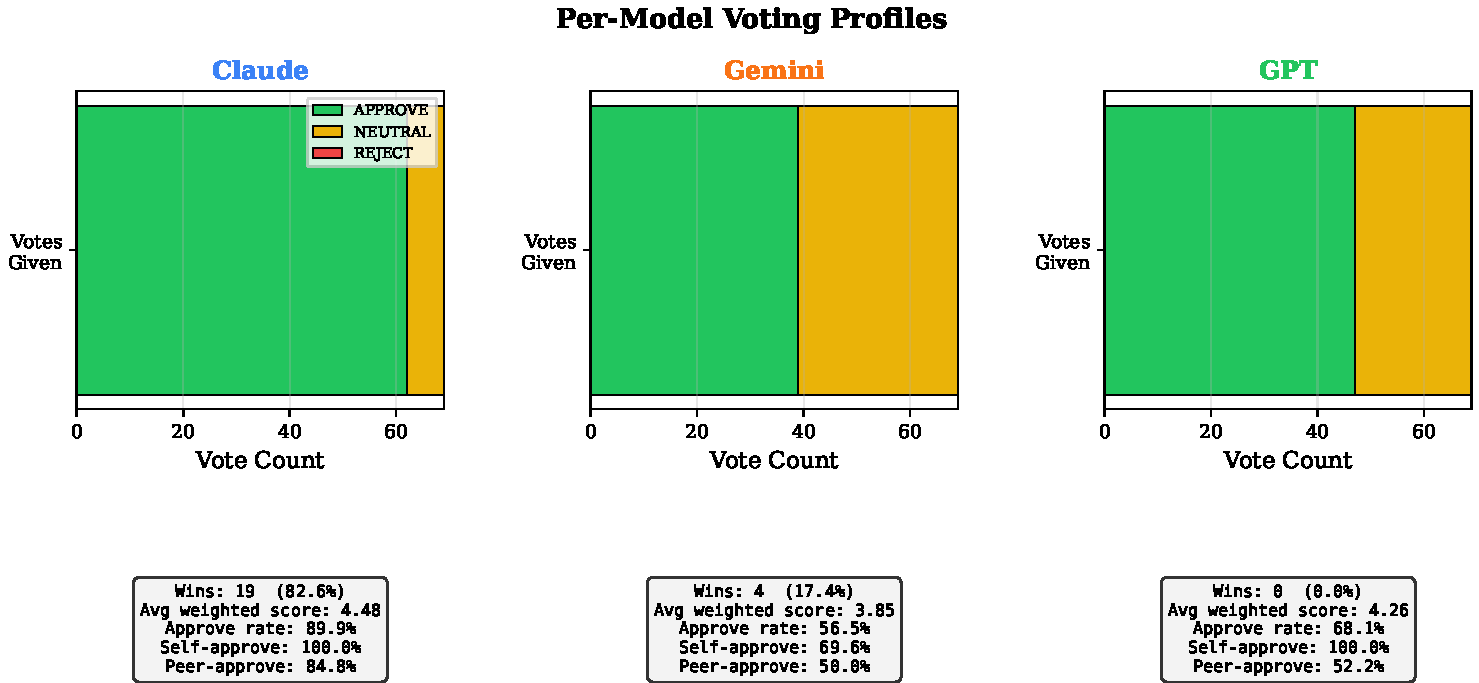
\includegraphics[width=\textwidth]{fig-model-profiles.pdf}
    \caption{Comparative model performance profiles across 16~deliberations. Each axis represents a distinct evaluation dimension: proposal win rate, mean peer approval score, REJECT votes cast, mean proposal length, and round-over-round change. The three models exhibit complementary strengths---Claude favors conservative, well-hedged proposals; GPT produces implementation-detailed specifications; Gemini excels at quantitative hardware-level analysis.}
    \label{fig:model_profiles}
\end{figure}

This diversity is a feature of the methodology, not a limitation, as illustrated in the comparative profiles shown in Fig.~\ref{fig:model_profiles}. Surowiecki's conditions for effective group judgment---diversity of opinion, independence of individual assessments, and decentralized knowledge~\cite{surowiecki2004wisdom}---are at least partially satisfied: the three model families have different architectures, training procedures, and RLHF approaches, providing a degree of diversity and independence not available from multiple instances of the same model. A deliberation panel composed of three instances of the same model would converge faster but explore a narrower design space. The complementary strengths---conservative risk assessment from Claude, implementation detail from GPT, quantitative hardware analysis from Gemini---produced structurally different trade studies than any single model could achieve alone, though we note this observation rests on the within-study comparison presented in Section~\ref{sec:validation_roadmap} rather than a formal controlled experiment.

\subsection{Limitations and Failure Modes}
\label{sec:limitations}

Five significant limitations were identified during the study.

\textbf{Sycophancy and framework adoption.} LLMs are known to exhibit sycophantic behavior---agreeing with prior statements rather than maintaining independent positions~\cite{perez2022sycophancy}.

\emph{Observation.} Of the 20~Round~2+ proposals across all multi-round deliberations, 14~(70\%) adopted the architectural framework of the previous round's winning proposal---incorporating its terminology, structural organization, or core design pattern---while only 6~(30\%) maintained an independent framework. In 11~of~14 cases where a Round~2 proposal adopted the Round~1 winner's framework, the Round~2 winning proposal was one that had done so.

\emph{Three competing interpretations.} (a)~\emph{Genuine quality recognition}: the winning framework was objectively better-suited to the problem, and models rationally adopted it after evaluation. The 13~REJECT votes cast across all deliberations indicate that models can and do express disagreement within this framework. (b)~\emph{Anchoring effect}: analogous to human Delphi studies~\cite{linstone1975delphi}, where panelists shown group medians shift their estimates toward the median in subsequent rounds. The 70\% framework adoption rate is comparable to the 60--80\% convergence rates documented in human Delphi panels. (c)~\emph{Sycophantic alignment}: an LLM-specific failure mode where models conform to prior context through pattern-matching rather than considered judgment.

\emph{What would distinguish them.} The $2\times2$ factorial design described in Section~\ref{sec:validation_roadmap} (Experiment~3) would isolate these effects. If convergence rates remain similar under blind conditions, interpretation~(a) is supported; if convergence slows substantially, interpretation~(c) is implicated; if convergence rates are intermediate, interpretation~(b) is most parsimonious.

\emph{Our assessment.} Without controlled data, we cannot distinguish between these interpretations. We note that in human Delphi studies, framework adoption rates of 60--80\% are common in later rounds and are generally interpreted as convergence rather than pathology. However, the mechanism differs: human experts adopt frameworks through considered judgment, while LLMs may do so through pattern-matching against prior context. This distinction is epistemologically significant and motivates the blind deliberation experiment as the highest-priority future work.

\textbf{Knowledge ceiling.} All three models share broadly similar training data, meaning that multi-model deliberation cannot compensate for systematic gaps in the training corpus. If no model has reliable knowledge about a specific topic (e.g., current asteroid mining economics), the deliberation will converge on a plausible but potentially incorrect consensus. The 8~divergent views identified as reflecting knowledge gaps (17\% of total) provide evidence of this limitation.

\textbf{Hallucinated citations.} Models occasionally cited non-existent papers or attributed findings to incorrect sources. While this is a well-documented LLM failure mode, it is particularly problematic in engineering deliberation where the credibility of a proposal may depend on cited evidence. We mitigated this through post-hoc citation verification, which identified 8~of~47 divergent views as reflecting knowledge gaps partly attributable to hallucinated supporting evidence.

\textbf{No repeated trials.} Each deliberation was conducted exactly once at temperature $T = 0.7$. Without repeated trials, we cannot estimate the variance of convergence statistics or determine whether the same divergent views would emerge across independent runs of the same question. The reported convergence statistics (mean 2.3~rounds, 95\% CI [1.9, 2.8] (bootstrap, 10,000 resamples, BCa method, computed across the 16 questions)) reflect variation \emph{across questions}, not across independent realizations of the same question. With $n=16$ and a discrete bounded outcome, this CI should be interpreted cautiously; the empirical distribution---4 questions in 1 round, 8 in 2 rounds, 2 in 3 rounds, 2 in 4 rounds---is more informative than the bootstrap interval. It is entirely possible that re-running a given deliberation would produce a different round winner, a different convergence trajectory, or different divergent views. Experiment~4 in Section~\ref{sec:validation_roadmap} specifies the required repeated-trials design.

\textbf{Governance and value-laden questions.} The methodology performed least well on questions involving governance structures and value judgments, where ``correct'' answers depend on normative assumptions rather than physical constraints. While the deliberation still produced useful output (comprehensive proposals, identified trade-offs), the convergence dynamics were meaningfully different: models converged on structural similarity (all proposed layered governance with checks and balances) while diverging on implementation details that reflected genuine value disagreements rather than technical uncertainties.

\subsection{Threats to Validity}
\label{sec:threats}

We identify five specific threats to the validity of the reported results, with estimated effect directions.

\textbf{Head truncation bias.} Prior-round proposals are truncated to the first 1{,}000~words before inclusion in subsequent-round prompts. This head truncation preserves introductory framing, design philosophy, and primary specifications while potentially losing detailed risk analysis, cost breakdowns, and secondary considerations. Effect direction: potentially inflated convergence speed and reduced diversity in later rounds, as models respond to similar introductory framings rather than the full proposals. Alternative truncation strategies (model-based summarization, section-weighted extraction) were not tested.

\textbf{Winner visibility and anchoring.} The deliberation protocol reveals the round winner's identity and score to all models in subsequent rounds. This creates a potential anchoring effect where models adjust their proposals toward the winning framework regardless of its objective merit. Effect direction: potentially inflated framework adoption rate (the observed 70\% in Round~2+ proposals) and artificially accelerated convergence. The blind deliberation experiment (Section~\ref{sec:validation_roadmap}, Experiment~3) is designed specifically to isolate this threat.

\textbf{Single synthesizer bias.} Using Claude~4.6 as the default synthesizer for conclusion documents introduces potential systematic bias: conclusions may overweight Claude's reasoning style, terminology preferences, or evaluation criteria relative to the other two models. Effect direction: conclusion documents may not reflect the full deliberation record with equal fidelity across all three model perspectives. Rotating the synthesizer role or using multi-model synthesis would mitigate this threat at the cost of additional API calls.

\textbf{Fixed temperature.} All deliberations were conducted at temperature $T = 0.7$ without sensitivity analysis. Lower temperatures may produce more conservative, deterministic proposals with faster convergence; higher temperatures may increase proposal diversity at the cost of coherence. The interaction between temperature and the voting mechanism's sensitivity to proposal variation is unknown. Effect direction: indeterminate without controlled comparison.

\textbf{JSON parsing failures.} Four of 48~Gemini voting instances (8.3\%) produced malformed JSON that defaulted to NEUTRAL. Post-hoc analysis indicates these were non-pivotal: in two cases the intended vote could be inferred from justification text (both APPROVE, making the default more conservative), and in the remaining two cases the winner margin exceeded 1.5~points. Effect direction: conservative bias in the affected rounds (NEUTRAL is lower than the likely intended APPROVE), but no effect on round winner identity.

\subsection{Epistemological Considerations}

The question ``what does consensus among LLMs mean?'' requires careful treatment. Multi-model agreement may reflect at least three distinct phenomena: (1)~convergence on objectively correct or well-established engineering knowledge, (2)~convergence on patterns common in training data regardless of their correctness, or (3)~sycophantic alignment driven by the deliberation structure itself. Our methodology cannot reliably distinguish between these three causes of agreement.

We argue that the divergent views are epistemically more valuable than the consensus. When models agree, the agreement may or may not reflect genuine engineering validity. When models disagree despite structured deliberation, the disagreement almost certainly identifies a genuine uncertainty---either in the engineering domain or in the models' knowledge. This is why we treat divergent views as first-class outputs and recommend that downstream engineering processes pay as much attention to preserved disagreements as to consensus conclusions.

Responsible framing is essential: outputs of this methodology should be characterized as ``AI-assisted preliminary trade studies'' rather than ``AI-validated engineering decisions.'' The methodology produces structured inputs for human engineering judgment; it does not replace that judgment.

% ============================================================
% 7. ETHICS STATEMENT
% ============================================================
\section{Ethics Statement}
\label{sec:ethics}

This work uses commercially available LLM APIs (Anthropic Claude, Google Gemini, OpenAI GPT) accessed through Databricks serving endpoints. No human subjects were involved in the deliberation process. The methodology is intended as a complement to human engineering judgment, not a replacement, and we recommend that outputs of multi-model deliberation always be reviewed by qualified domain experts before informing engineering decisions.

We acknowledge four ethical considerations specific to this work. First, the use of LLMs for engineering trade studies may create a false sense of authority if outputs are presented without appropriate caveats about the methodology's limitations. We address this by requiring that all deliberation outputs carry metadata identifying them as AI-generated preliminary analyses. Second, the methodology could be misused to justify predetermined conclusions by selectively reporting consensus while ignoring divergent views; the structured divergent views schema is designed partly to prevent this by making disagreements as visible as agreements. Third, this paper was itself produced with AI writing assistance; the research design, implementation, and analysis were conducted by the Project Dyson research team with AI tools used for drafting and revision. Fourth, the computational cost of running frontier LLMs through multi-round deliberation, while modest for individual questions (\$5--20 per deliberation), has non-trivial energy implications at scale. An organization applying this methodology to hundreds of trade studies would incur meaningful computational energy consumption, which should be weighed against the value of the outputs and compared with the environmental footprint of equivalent human expert travel and coordination.

The deliberation system and all outputs are released as open-source software under permissive licensing, enabling independent reproduction, auditing, and extension by the research community.

% ============================================================
% 8. CONCLUSION
% ============================================================
\section{Conclusion}
\label{sec:conclusion}

We have presented a structured methodology for multi-model AI deliberation on complex engineering decisions, specifying round structure, weighted voting mechanics, multi-pathway termination conditions, and a divergent views schema in sufficient detail for independent reproduction. Illustrative application to 16~architectural trade studies illustrates the methodology's operational feasibility: deliberations terminate in 1--4 rounds, the voting mechanism surfaces substantive technical disagreements, and the divergent views schema captures trade-offs across heterogeneous engineering domains. Two baseline comparisons---aggregation-only synthesis (Section~\ref{sec:aggregation}) and single-model self-refinement (Section~\ref{sec:self_refinement})---provide initial evidence about the deliberation mechanism's contribution, though both comparisons have important limitations.

The self-refinement baseline (Section~\ref{sec:self_refinement}) is particularly instructive. On a stratified sample of four questions, a single model iterating through generate-critique-refine loops produced conclusions with identical structural metrics to multi-model deliberation (6~key points, 4~unresolved questions, 5~recommended actions per question). This structural equivalence likely reflects prompt template conformity rather than analytical equivalence, but it underscores that structural metrics alone cannot distinguish between conditions. Qualitative differences---absence of genuine adversarial challenges, missing cross-model knowledge contributions, and convergence on single analytical frameworks---were observable but not quantified. Whether these qualitative differences translate to better engineering decisions remains an open empirical question requiring expert evaluation.

The methodology's most distinctive contribution is its treatment of disagreement as information rather than noise. Where conventional consensus methods seek to minimize dispersion, our system preserves divergent views in a structured schema with model attribution, supporting evidence, and resolution status. Of the 47~divergent topics identified, 12 were confirmed as genuine engineering trade-offs by targeted literature review, and 19~represented reasonable judgment calls where the literature provides no definitive guidance. These 31~substantive disagreements (66\% of total) represent design space that single-model self-refinement---which lacks the adversarial dynamics necessary to surface genuine architectural alternatives---would likely not have surfaced independently.

This paper contributes a structured methodology and open-source implementation for multi-model engineering deliberation. The methodology's most distinctive feature---preservation of disagreements as machine-readable artifacts---addresses a gap in both multi-agent AI systems and engineering design practice. Illustrative application to 16~trade studies illustrates operational feasibility, and preliminary baseline comparisons (aggregation-only and self-refinement) provide initial context, but full empirical validation requires the remaining controlled comparisons identified in Section~\ref{sec:validation_roadmap}: blind deliberation for sycophancy assessment, repeated trials for variance estimation, and expert evaluation of output quality across conditions. The modest cost of these experiments (\$260--1{,}060 in API costs) underscores that the primary barrier to validation is experimental design effort, not resource constraints; we encourage independent research groups to conduct these comparisons.

Multi-model AI deliberation is not a replacement for human engineering expertise. It is a tractable method for rapidly generating structured, adversarially reviewed, and explicitly documented preliminary trade studies---producing inputs for human engineering judgment across a broad space of architectural questions.

% ============================================================
% ACKNOWLEDGMENTS
% ============================================================
\section*{Acknowledgments}

The authors thank the open-source community contributors to Project Dyson for providing the engineering context and research questions that motivated this work. Computational resources for LLM API access were provided through Databricks serving endpoints.

% ============================================================
% DATA AVAILABILITY
% ============================================================
\section*{Data Availability}

The complete deliberation system implementation (orchestration code, prompt templates, configuration), full deliberation transcripts, voting records, conclusions, and divergent views for all 16~trade studies are available as open-source at the Project Dyson repository. Interactive exploration of results is available at \url{https://projectdyson.org}.

% ============================================================
% REFERENCES
% ============================================================
\begin{thebibliography}{99}

\bibitem{linstone1975delphi}
H.~A. Linstone and M.~Turoff, \emph{The Delphi Method: Techniques and Applications}. Addison-Wesley, 1975.

\bibitem{dalkey1963experimental}
N.~Dalkey and O.~Helmer, ``An experimental application of the Delphi method to the use of experts,'' \emph{Management Science}, vol.~9, no.~3, pp.~458--467, 1963.

\bibitem{janis1982groupthink}
I.~L. Janis, \emph{Groupthink: Psychological Studies of Policy Decisions and Fiascoes}, 2nd~ed. Houghton Mifflin, 1982.

\bibitem{irving2018debate}
G.~Irving, C.~Christiano, and D.~Amodei, ``AI safety via debate,'' \emph{arXiv preprint arXiv:1805.00899}, 2018.

\bibitem{du2023debate}
Y.~Du, S.~Li, A.~Torralba, J.~B. Tenenbaum, and I.~Mordatch, ``Improving factuality and reasoning in language models through multiagent debate,'' in \emph{Proc.\ International Conference on Machine Learning (ICML)}, 2023.

\bibitem{wu2023autogen}
Q.~Wu, G.~Bansal, J.~Zhang, Y.~Wu, B.~Li, E.~Zhu, L.~Jiang, X.~Zhang, S.~Zhang, J.~Liu, A.~H.~Awadallah, R.~W.~White, D.~Burger, and C.~Wang, ``AutoGen: Enabling next-gen LLM applications via multi-agent conversation,'' \emph{arXiv preprint arXiv:2308.08155}, 2023.

\bibitem{zheng2024judging}
L.~Zheng, W.-L. Chiang, Y.~Sheng, S.~Zhuang, Z.~Wu, Y.~Zhuang, Z.~Lin, Z.~Li, D.~Li, E.~P. Xing, H.~Zhang, J.~E. Gonzalez, and I.~Stoica, ``Judging LLM-as-a-judge with MT-Bench and Chatbot Arena,'' in \emph{Advances in Neural Information Processing Systems (NeurIPS)}, 2023.

\bibitem{bubeck2023sparks}
S.~Bubeck, V.~Chandrasekaran, R.~Eldan, J.~Gehrke, E.~Horvitz, E.~Kamar, P.~Lee, Y.~T. Lee, Y.~Li, S.~Lundberg, H.~Nori, H.~Palangi, M.~T. Ribeiro, and Y.~Zhang, ``Sparks of artificial general intelligence: Early experiments with GPT-4,'' \emph{arXiv preprint arXiv:2303.12712}, 2023.

\bibitem{openai2024gpt4}
OpenAI, ``GPT-4 technical report,'' \emph{arXiv preprint arXiv:2303.08774}, 2024.

\bibitem{bai2022constitutional}
Y.~Bai, S.~Kadavath, S.~Kundu, A.~Askell, J.~Kernion, A.~Jones, A.~Chen, A.~Goldie, A.~Mirhoseini, C.~McKinnon, et~al., ``Constitutional AI: Harmlessness from AI feedback,'' \emph{arXiv preprint arXiv:2212.08073}, 2022.

\bibitem{perez2022sycophancy}
E.~Perez, S.~Ringer, K.~Luko\v{s}i\={u}t\.{e}, K.~Nguyen, E.~Chen, S.~Heiner, C.~Pettit, C.~Olsson, S.~Kundu, S.~Kadavath, et~al., ``Discovering language model behaviors with model-written evaluations,'' in \emph{Findings of ACL}, 2023.

\bibitem{mcdermott1982r1}
J.~McDermott, ``R1: A rule-based configurer of computer systems,'' \emph{Artificial Intelligence}, vol.~19, no.~1, pp.~39--88, 1982.

\bibitem{autodesk2023generative}
Autodesk Research, ``Generative design: An overview,'' Autodesk, Tech.\ Rep., 2023.

\bibitem{arulmohan2023extracting}
S.~Arulmohan, M.-J.~Meurs, and S.~Mosser, ``Extracting domain models from textual requirements in the era of large language models,'' in \emph{Proc.\ ACM/IEEE Int. Conf. Model Driven Eng. Languages Syst. Companion (MODELS-C)}, 2023.

\bibitem{chen2021codex}
M.~Chen, J.~Tworek, H.~Jun, Q.~Yuan, H.~Pinto de Oliveira, J.~Kaplan, H.~Edwards, Y.~Burda, N.~Joseph, G.~Brockman, et~al., ``Evaluating large language models trained on code,'' \emph{arXiv preprint arXiv:2107.03374}, 2021.

\bibitem{delbecq1975group}
A.~L. Delbecq, A.~H. Van~de~Ven, and D.~H. Gustafson, \emph{Group Techniques for Program Planning: A Guide to Nominal Group and Delphi Processes}. Scott Foresman, 1975.

\bibitem{fitch2001rand}
K.~Fitch, S.~J. Bernstein, M.~D. Aguilar, B.~Burnand, J.~R. LaCalle, J.~P. L\'{a}zaro, M.~van~het~Loo, J.~McDonnell, J.~Vader, and J.~P. Kahan, \emph{The RAND/UCLA Appropriateness Method User's Manual}. RAND Corporation, 2001.

\bibitem{zenko2015red}
M.~Zenko, \emph{Red Team: How to Succeed by Thinking Like the Enemy}. Basic Books, 2015.

\bibitem{schwenk1990effects}
C.~R. Schwenk, ``Effects of devil's advocacy and dialectical inquiry on decision making: A meta-analysis,'' \emph{Organizational Behavior and Human Decision Processes}, vol.~47, no.~1, pp.~161--176, 1990.

\bibitem{schwartz1996art}
P.~Schwartz, \emph{The Art of the Long View: Planning for the Future in an Uncertain World}. Currency Doubleday, 1996.

\bibitem{barnhart2007smallsat}
D.~J. Barnhart, T.~Vladimirova, and M.~N. Sweeting, ``Very-small-satellite design for distributed space missions,'' \emph{Journal of Spacecraft and Rockets}, vol.~44, no.~6, pp.~1294--1306, 2007.

\bibitem{ostrom1990governing}
E.~Ostrom, \emph{Governing the Commons: The Evolution of Institutions for Collective Action}. Cambridge University Press, 1990.

\bibitem{brambilla2013swarm}
M.~Brambilla, E.~Ferrante, M.~Birattari, and M.~Dorigo, ``Swarm robotics: A review from the swarm engineering perspective,'' \emph{Swarm Intelligence}, vol.~7, no.~1, pp.~1--41, 2013.

\bibitem{incose2023handbook}
INCOSE, \emph{Systems Engineering Handbook}, 5th~ed. International Council on Systems Engineering, 2023.

\bibitem{nasa2020se}
NASA, ``NASA Systems Engineering Handbook,'' NASA SP-2016-6105 Rev.~2, 2020.

\bibitem{liang2024encouraging}
T.~Liang, Z.~He, W.~Jiao, X.~Wang, Y.~Wang, R.~Wang, Y.~Yang, Z.~Tu, and S.~Shi, ``Encouraging divergent thinking in large language models through multi-agent debate,'' \emph{arXiv preprint arXiv:2305.19118}, 2024.

\bibitem{chan2024chateval}
C.~M. Chan, W.~Chen, Y.~Su, J.~Yu, W.~Xue, S.~Zhang, J.~Fu, and Z.~Liu, ``ChatEval: Towards better LLM-based evaluators through multi-agent debate,'' \emph{arXiv preprint arXiv:2308.07201}, 2023.

\bibitem{wang2024rethinking}
Q.~Wang, Z.~Wang, Y.~Su, H.~Tong, and Y.~Song, ``Rethinking the bounds of LLM reasoning: Are multi-agent discussions the key?,'' \emph{arXiv preprint arXiv:2402.18272}, 2024.

\bibitem{surowiecki2004wisdom}
J.~Surowiecki, \emph{The Wisdom of Crowds: Why the Many Are Smarter Than the Few and How Collective Wisdom Shapes Business, Economies, Societies, and Nations}. Doubleday, 2004.

\bibitem{keeney1976decisions}
R.~L. Keeney and H.~Raiffa, \emph{Decisions with Multiple Objectives: Preferences and Value Tradeoffs}. John Wiley \& Sons, 1976.

\bibitem{kadavath2022language}
S.~Kadavath, T.~Conerly, A.~Askell, T.~Henighan, D.~Drain, E.~Perez, N.~Schiefer, Z.~Hatfield-Dodds, N.~DasSarma, E.~Tran-Kemp, et~al., ``Language models (mostly) know what they know,'' \emph{arXiv preprint arXiv:2207.05221}, 2022.

\bibitem{lee1991drl}
J.~Lee and K.-Y. Lai, ``What's in design rationale?,'' \emph{Human--Computer Interaction}, vol.~6, no.~3--4, pp.~251--280, 1991.

\bibitem{maclean1991qoc}
A.~MacLean, R.~M. Young, V.~M.~E. Bellotti, and T.~P. Moran, ``Questions, options, and criteria: Elements of design space analysis,'' \emph{Human--Computer Interaction}, vol.~6, no.~3--4, pp.~201--250, 1991.

\bibitem{pugh1991total}
S.~Pugh, \emph{Total Design: Integrated Methods for Successful Product Engineering}. Addison-Wesley, 1991.

\bibitem{saaty1980ahp}
T.~L. Saaty, \emph{The Analytic Hierarchy Process: Planning, Priority Setting, Resource Allocation}. McGraw-Hill, 1980.

\bibitem{madaan2023self}
A.~Madaan, N.~Tandon, P.~Gupta, S.~Halber, L.~Gao, S.~Wiegreffe, U.~Alon, N.~Dziri, S.~Prabhumoye, Y.~Yang, S.~Gupta, B.~P. Majumder, H.~Yazdanbakhsh, and P.~Clark, ``Self-Refine: Iterative refinement with self-feedback,'' in \emph{Advances in Neural Information Processing Systems (NeurIPS)}, 2023.

\end{thebibliography}

\end{document}
